%% ============================================================
%%  docs/gpu_octree_meshing.tex
%%  From CPU SDF shape construction to GPU-resident Surface Nets
%%  meshing and rendering.
%% ============================================================
\documentclass[11pt,a4paper]{article}

\usepackage[T1]{fontenc}
\usepackage[utf8]{inputenc}
\usepackage{lmodern}
\usepackage{microtype}
\usepackage[a4paper,left=2.2cm,right=2.2cm,top=2.5cm,bottom=2.5cm]{geometry}
\usepackage{amsmath,amssymb,amsthm}
\usepackage{mathtools}
\usepackage{xcolor}
\usepackage{graphicx}
\usepackage{booktabs,longtable,array}
\usepackage{hyperref}
\usepackage{cleveref}
\usepackage{float}
\usepackage{caption}
\usepackage{subcaption}
\usepackage{enumitem}
\usepackage{multicol}
\usepackage{fancyhdr}
\usepackage{tcolorbox}
\usepackage{algorithm}
\usepackage{algpseudocode}
\usepackage{listings}
\usepackage{tikz}
\usetikzlibrary{arrows.meta,positioning,shapes.geometric,fit,calc,
  decorations.pathreplacing,backgrounds,patterns.meta,chains}
\usepackage{pgfplots}
\pgfplotsset{compat=1.18}

\definecolor{ink}{RGB}{26,34,48}
\definecolor{accent}{RGB}{24,92,168}
\definecolor{accent2}{RGB}{196,86,30}
\definecolor{soft}{RGB}{238,242,247}
\definecolor{good}{RGB}{28,120,74}

\hypersetup{
  colorlinks=true,
  linkcolor=accent,
  citecolor=accent2,
  urlcolor=accent,
  pdftitle={From CPU SDF Shapes to GPU-Resident Surface Nets Meshing},
  pdfauthor={Vulkan Engine Technical Report}
}

\captionsetup{font=small,labelfont=bf,justification=raggedright,
  singlelinecheck=false}
\setlist{nosep,leftmargin=1.5em}
\setlength{\parskip}{2.5pt}
\setlength{\emergencystretch}{3.5em}
\setlength{\parindent}{0pt}
\linespread{1.06}

\pagestyle{fancy}
\fancyhf{}
\fancyhead[L]{\small CPU SDF Octree $\rightarrow$ GPU Surface Nets}
\fancyhead[R]{\small Technical Report}
\fancyfoot[C]{\thepage}
\renewcommand{\headrulewidth}{0.4pt}

\newcommand{\code}[1]{\texttt{\detokenize{#1}}}
\newcommand{\sdf}{\operatorname{SDF}}
\newcommand{\interp}{\operatorname{interp}}
\newcommand{\clip}{\operatorname{clamp}}
\newcommand{\argmin}{\operatorname*{arg\,min}}
\newcommand{\R}{\mathbb{R}}
\newcommand{\V}{\mathcal{V}}
\newcommand{\T}{\mathcal{T}}
\newcommand{\N}{\mathcal{N}}
\newcommand{\Oh}{\mathcal{O}}
\newcommand{\dd}{\,\mathrm{d}}

\newtheorem{definition}{Definition}
\newtheorem{proposition}{Proposition}
\newtheorem{invariant}{Invariant}
\newtheorem{remark}{Remark}

\tikzset{
  box/.style={draw=ink!55,fill=soft,rounded corners=2pt,
    align=center,font=\small,inner sep=5pt,minimum height=8mm},
  cpu/.style={box,fill=blue!8,draw=accent!65},
  gpu/.style={box,fill=orange!9,draw=accent2!70},
  io/.style={box,fill=green!8,draw=good!60},
  arrow/.style={-{Latex[length=2.2mm]},thick,draw=ink!70},
  darrow/.style={-{Latex[length=2.2mm]},thick,dashed,draw=ink!55},
  note/.style={font=\scriptsize,text=ink!80,align=center},
  grid/.style={draw=ink!18,line width=0.35pt}
}

\lstdefinestyle{cpp}{
  language=C++,
  basicstyle=\ttfamily\scriptsize,
  keywordstyle=\color{accent!85!black}\bfseries,
  commentstyle=\color{gray!65},
  stringstyle=\color{accent2!80!black},
  numberstyle=\tiny\color{gray},
  numbers=left,numbersep=5pt,
  breaklines=true,tabsize=2,showstringspaces=false,
  frame=single,rulecolor=\color{ink!18},
  backgroundcolor=\color{ink!2},
  captionpos=b,
  columns=fullflexible,keepspaces=true
}
\lstdefinestyle{glsl}{
  language=C,
  basicstyle=\ttfamily\scriptsize,
  keywordstyle=\color{accent!85!black}\bfseries,
  commentstyle=\color{gray!65},
  numberstyle=\tiny\color{gray},
  numbers=left,numbersep=5pt,
  breaklines=true,tabsize=2,showstringspaces=false,
  frame=single,rulecolor=\color{ink!18},
  backgroundcolor=\color{ink!2},
  captionpos=b,
  columns=fullflexible,keepspaces=true
}
\lstset{style=cpp}

\newtcolorbox{keybox}[1][]{
  colback=soft,colframe=accent!55,boxrule=0.6pt,arc=2pt,
  left=6pt,right=6pt,top=4pt,bottom=4pt,
  fonttitle=\bfseries\small,title={#1}
}

\title{%
  \vspace{-1.2cm}
  \textbf{From CPU SDF Shapes to GPU-Resident Surface Nets Meshing}\\[4pt]
  {\large A Detailed Account of Adaptive Octree Construction,\\
  GPU Topology Extraction, and Real-Time Rendering}\\[8pt]
  {\normalsize Vulkan Engine Technical Report}
}
\author{Henrique Rocha}
\date{\today}

\begin{document}
\maketitle
\thispagestyle{empty}

\begin{abstract}
This report describes, end to end, how the engine turns an implicit
signed-distance-model (SDF) scene into a rendered, crack-free, adaptive
triangle mesh.  The construction is deliberately split between two
processors.  The CPU owns the \emph{semantic} structure: it evaluates the
model's distance field, builds and edits an adaptive octree of corner
samples, chooses the level-of-detail (LoD) ladder, and publishes chunk
metadata.  The GPU owns every \emph{Cartesian} operation: it flattens a
chunk's octree neighbourhood into compact tables, walks the twelve cube
edges, stitches LoD discontinuities, solves one dual vertex per surface
cell, emits the triangle stream, and writes the final 64-byte vertex and
index payloads directly into the renderer's device-local packed pools.
No runtime vertex is read back to the host.

The document is organised as a sequence of algorithms with the data
structures and invariants that make them correct.  It covers the SDF and
CSG foundations, octree storage and threading, the CPU shape recursion,
simplification and the chunk ladder, the CPU reference walker used by the
offline exporter, the exact GPU port in \code{OctreeTriangles.comp}, the
single-dispatch host orchestration, packed-pool span binding and alignment,
GPU culling with a hole-free hierarchical LoD gate, shadows and ray
tracing, GPU-side vegetation and lava effects, and the synchronization and
validation rules that keep the pipeline clean.  It closes with measured
costs, memory budgets, failure modes, and a set of correctness invariants
that a future change must preserve.
\end{abstract}

\vspace{0.5em}
\noindent\textbf{Keywords:} signed distance functions; adaptive octree;
Surface Nets; dual contouring; GPU meshing; compute shaders; level of
detail; crack-free stitching; Vulkan; indirect rendering.

\tableofcontents
\listoffigures
\listoftables
\listofalgorithms

\newpage
\section*{Notation and conventions}
\addcontentsline{toc}{section}{Notation and conventions}

\begin{longtable}{@{}p{0.22\linewidth}p{0.70\linewidth}@{}}
\toprule
Symbol & Meaning\\
\midrule
$f(\mathbf{x})$ & signed distance field; negative inside the solid\\
$\V$ & an adaptive octree node/cell\\
$\mathbf{c}$ & a cube minimum corner $\mathbf{c}\in\R^3$\\
$L$ & cube edge length\\
$C_i$ & cube corner $i$; bits $(x,y,z)$ with bit 2 $=x$, bit 1 $=y$, bit 0 $=z$\\
$d_i$ & stored SDF sample at corner $i$; $+\infty$ means ``no data''\\
$\T$ & a triangle (three corners / three dual vertices)\\
$s$ & a surface-node slot index assigned on the host\\
$\N$ & a flattened node table uploaded for one chunk\\
$\mathcal{P}_v,\mathcal{P}_i$ & packed vertex and index pools\\
$b_v,b_i$ & pool element base of a reserved chunk span\\
$\Delta$ & one chunk's cube edge (the chunk boundary)\\
$r$ & LoD rung index; $r=0$ is the finest published rung\\
$\tau$ & a threshold (simplification error, break epsilon, etc.)\\
\bottomrule
\end{longtable}

\noindent
The reader is assumed to know Vulkan at the level of command buffers,
descriptor sets, compute dispatches, and pipeline barriers.  The report
does not repeat the Vulkan specification; it explains why each operation
is placed where it is and which synchronization argument makes it legal.

\section{Introduction}
\label{sec:intro}

\subsection{The problem}

A modern terrain and solid-geometry engine must satisfy four requirements
at the same time:

\begin{enumerate}[label=\textbf{R\arabic*.},leftmargin=2.2em]
\item \textbf{Authoring freedom.}  Designers describe geometry with
  implicit primitives, Boolean operations, noise, and material painters,
  not with a fixed triangle list.
\item \textbf{Adaptive detail.}  Near geometry must be finely tessellated;
  the same region observed from a kilometre away must collapse to a coarse
  representation without cracks or holes.
\item \textbf{Low host traffic.}  A terrain that streams hundreds of
  chunks per second cannot afford a GPU$\rightarrow$CPU$\rightarrow$GPU
  round trip for every vertex.
\item \textbf{Real-time rendering.}  The result must feed frustum culling,
  shadow cascades, ray tracing, vegetation placement, and volumetric
  effects without a second geometry representation.
\end{enumerate}

The engine answers with a split pipeline.  The CPU evaluates the scene's
signed distance field (SDF) and maintains an adaptive octree of corner
samples.  It never stores a triangle mesh.  The GPU receives a flattened
subset of that octree for one chunk, performs the full adaptive Surface
Nets walk, solves one dual vertex per surface cell, and writes the
resulting vertices and indices directly into the renderer's persistent
packed pools.  The host sees integer counters, not positions.

\begin{figure}[htbp]
\centering
\resizebox{\linewidth}{!}{%
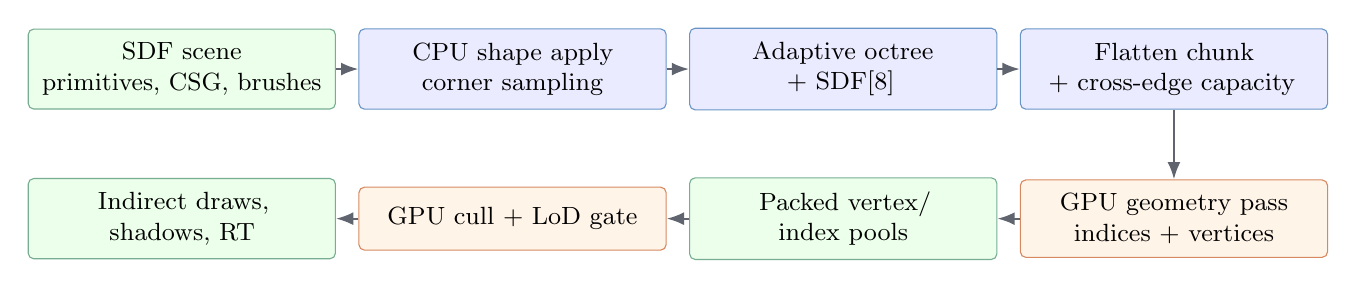
\begin{tikzpicture}[x=1cm,y=1cm,font=\small,every node/.append style={text width=3.55cm}]
  \node[io]  (author)  at (0.0,3.1) {SDF scene\\primitives, CSG, brushes};
  \node[cpu] (apply)   at (4.2,3.1) {CPU shape apply\\corner sampling};
  \node[cpu] (tree)    at (8.4,3.1) {Adaptive octree\\+ SDF[8]};
  \node[cpu] (flat)    at (12.6,3.1) {Flatten chunk\\+ cross-edge capacity};
  \node[gpu] (mesh)    at (12.6,1.2) {GPU geometry pass\\indices + vertices};
  \node[io]  (pools)   at (8.4,1.2) {Packed vertex/\\index pools};
  \node[gpu] (cull)    at (4.2,1.2) {GPU cull + LoD gate};
  \node[io]  (frame)   at (0.0,1.2) {Indirect draws,\\shadows, RT};
  \draw[arrow] (author)--(apply);
  \draw[arrow] (apply)--(tree);
  \draw[arrow] (tree)--(flat);
  \draw[arrow] (flat)--(mesh);
  \draw[arrow] (mesh)--(pools);
  \draw[arrow] (pools)--(cull);
  \draw[arrow] (cull)--(frame);
\end{tikzpicture}}
\caption{End-to-end pipeline.  Blue nodes execute on the CPU; orange nodes
execute on the GPU.  The only data crossing from GPU to CPU are integer
counters used for span sizing and statistics.  Chunk geometry itself never
returns to the host.}
\label{fig:pipeline}
\end{figure}

\subsection{Why not mesh on the CPU?}

The original engine did exactly that.  \code{Octree::iterateTriangles}
walked the tree, solved QEF vertices, and appended triangles to a
\code{Geometry} object; a staging copy then uploaded the vertex and index
arrays.  The CPU path is still present as
\code{OctreeTriangleTessellator}, but it now serves only the offline
Blender exporter.  Moving the same walk to a compute shader produced three
concrete benefits:

\begin{itemize}
\item \textbf{The host never touches the vertex stream.}  A chunk's
  topology is written into a device-local span.  The host reserves the
  span, publishes a draw command, and never reads a position.
\item \textbf{The adaptive walk parallelises trivially.}  One invocation
  owns one scan cell.  All per-cell state (break lists, QEF memo, recursion
  stack) is private, so the only atomics are the index append, the overflow
  counters, and the per-node vertex-writer election.
\item \textbf{The renderer and the mesher share one memory layout.}  The
  compute pass writes the renderer's exact 64-byte \code{Vertex} format
  and chunk-local index values.  There is no conversion, compaction, or
  intermediate mesh object.
\end{itemize}

The cost is that the GPU must see exactly the octree neighbourhood the CPU
walker would have traversed: coarser neighbours for edge stitching, finer
children for the descent, the world-root path, and a deterministic
assignment of vertex slots.  The bulk of this report is about making that
flattening exact and about the single-pass GPU mesher that consumes it.

\subsection{Contributions}

This report makes the following contributions, all implemented in the
current engine:

\begin{enumerate}[label=\textbf{C\arabic*.},leftmargin=2.2em]
\item A precise description of the CPU octree as a \emph{corner-sample
  store}, including its +1-shifted LoD representation, block allocator,
  quadratic-error simplification, and threaded \code{apply} recursion.
\item A root-consistent flattening algorithm that turns a chunk's octree
  neighbourhood into eight compact storage buffers and a scan-cell list,
  with host-assigned vertex slots packed into node flags.
\item A single-pass GPU topology geometry stage: the CPU cross-edge count
  sizes both spans, and one dispatch appends the chunk-local index stream
  and writes each referenced vertex payload exactly once.
\item Per-chunk cross-edge capacity accounting and overflow growth: an
  overflow is reported without out-of-bounds writes and grows only the
  affected chunk's span.
\item An exact GPU port of the adaptive edge stitching algorithm
  (per-edge break collection at LoD boundaries), including its fixed
  capacities, overflow policy, and deterministic ordering.
\item A packed-pool span protocol that binds only a chunk's slice of a
  large pool, respects \code{maxStorageBufferRange}, handles alignment
  padding, and publishes the draw entry only when the fence signals.
\item A hole-free hierarchical LoD gate used by the raster, shadow,
  bounding-box, and water streams, plus the GPU-resident effect consumers
  (vegetation instances and lava/fire anchors) that read the same chunk
  metadata.
\item A validation-oriented account of the synchronization, lifetime, and
  determinism rules that keep the path clean across asynchronous compute,
  graphics, and transfer queues.
\end{enumerate}

\subsection{Reading guide}

\Cref{sec:foundations}--\ref{sec:cpuwalk} cover the CPU side:
SDF mathematics, octree storage, the shape recursion, simplification, and
the reference walker.  \Cref{sec:gpudesign}--\ref{sec:finalize} cover the
GPU meshing pass in increasing detail.  \Cref{sec:orch}--\ref{sec:sync}
cover host orchestration and synchronization.  \Cref{sec:render}--
\ref{sec:effects} follow the mesh into rendering and effects.
\Cref{sec:perf}--\ref{sec:validation} give measured costs and correctness
invariants.  Appendices contain the exact tables and storage layouts.

\begin{keybox}[The one-sentence summary]
The CPU decides \emph{what the surface is}; the GPU decides \emph{where
its vertices are} and writes them once, directly into the buffers the
renderer already owns.
\end{keybox}

\section{Foundations and related work}
\label{sec:foundations}

\subsection{Implicit surfaces and signed distance fields}

A signed distance field assigns to every point $\mathbf{x}\in\R^3$ the
signed Euclidean distance to the boundary $\partial\Omega$ of a solid
$\Omega$:
\begin{equation}
  f(\mathbf{x}) =
  \begin{cases}
    +\operatorname{dist}(\mathbf{x},\partial\Omega), & \mathbf{x}\notin\Omega,\\[2pt]
    -\operatorname{dist}(\mathbf{x},\partial\Omega), & \mathbf{x}\in\Omega.
  \end{cases}
  \label{eq:sdf}
\end{equation}
The surface is the zero set $f^{-1}(0)$.  The gradient of a true distance
field has unit length and points away from the solid, so the unit normal is
\begin{equation}
  \mathbf{n}(\mathbf{x}) = \frac{\nabla f(\mathbf{x})}{\|\nabla f(\mathbf{x})\|}.
  \label{eq:normal}
\end{equation}
The engine stores only eight corner samples per octree cell and
reconstructs $f$ inside the cell by trilinear interpolation.  This is a
deliberate approximation: it makes the field cheap to evaluate, cheap to
cache, and identical between the CPU reference and the GPU shader.

\subsection{CSG operations}

A CSG operation combines two distance fields.  The engine supports union,
subtraction, intersection, and a generic user operation.  For two fields
$f_1,f_2$ the common rules are
\begin{align}
  \text{union}:&\quad \min(f_1,f_2), \label{eq:union}\\
  \text{intersection}:&\quad \max(f_1,f_2), \label{eq:intersection}\\
  \text{subtraction}:&\quad \max(f_1,-f_2). \label{eq:subtraction}
\end{align}
The exact expressions are not distance fields in the strict sense after
subtraction (the result can be negative in the subtracted volume), but they
preserve the zero set and the sign, which is all the mesher needs.  The
engine also supports smooth minima and custom effects; those change the
field values but not the extraction algorithm.

\begin{figure}[htbp]
\centering
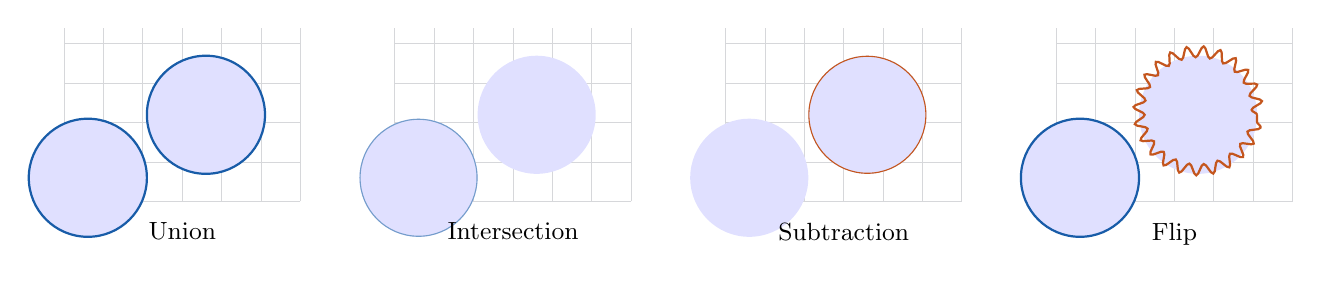
\begin{tikzpicture}[scale=1.0]
  \foreach \dx/\lab in {0/Union, 4.2/Intersection, 8.4/Subtraction, 12.6/Flip} {
    \begin{scope}[shift={(\dx,0)}]
      \draw[grid] (0,0) grid[step=0.5] (3,2.2);
      \fill[blue!12] (0.3,0.3) circle (0.75);
      \fill[blue!12] (1.8,1.1) circle (0.75);
      \ifdim\dx pt=0pt
        \draw[accent,thick] (0.3,0.3) circle (0.75);
        \draw[accent,thick] (1.8,1.1) circle (0.75);
      \fi
      \ifdim\dx pt=4.2pt
        \begin{scope}
          \clip (0.3,0.3) circle (0.75);
          \fill[accent2!25] (1.8,1.1) circle (0.75);
          \draw[accent!60,thick] (0.3,0.3) circle (0.75);
          \draw[accent2,thick] (1.8,1.1) circle (0.75);
        \end{scope}
      \fi
      \ifdim\dx pt=8.4pt
        \begin{scope}
          \clip (1.8,1.1) circle (0.75);
          \fill[white] (0.3,0.3) circle (0.75);
          \draw[accent!60,thick] (0.3,0.3) circle (0.75);
          \draw[accent2,thick] (1.8,1.1) circle (0.75);
        \end{scope}
      \fi
      \ifdim\dx pt=12.6pt
        \draw[accent,thick] (0.3,0.3) circle (0.75);
        \draw[accent2,thick,decorate,
          decoration={snake,amplitude=0.7mm,segment length=2mm}] (1.8,1.1) circle (0.75);
      \fi
      \node[below,font=\small] at (1.5,-0.15) {\lab};
    \end{scope}
  }
\end{tikzpicture}
\caption{Two-dimensional cross-sections of the CSG rules.  Blue is the
solid; a subtraction removes the second field from the first; the rightmost
panel illustrates a non-distance-preserving effect whose zero set and sign
are still well defined.}
\label{fig:csg}
\end{figure}

\subsection{Dual contouring and Surface Nets}

Marching Cubes places one vertex on each sign-changing cube edge and
connects them inside the cube.  Dual methods instead place \emph{one}
vertex per surface cell and connect the vertices of cells that share an
edge.  The resulting mesh is the dual of the cell complex.  Surface Nets
use an average of edge crossings; Dual Contouring solves a quadratic error
function (QEF) to place a vertex that fits the sampled Hermite data
(position and normal on each crossing edge).

The engine uses a QEF solve (with a mass-point regularizer) to place one
vertex per surface cell, then extracts triangles by scanning the twelve
edges of each scan cell.  The method is often called ``dual contouring'',
but the extraction rule is the Surface Nets ring rule: for each active
edge, collect the four cells around the edge, keep the surface cells,
order them around the edge, and triangulate the resulting three- or
four-gon.  The QEF is what makes the vertex position smooth; the ring rule
is what makes the connectivity exact and crack-free.

\subsection{Adaptive octrees and LoD}

A uniform dual grid at the finest resolution is wasteful: terrain near the
camera needs centimetres, while a distant ridge needs tens of metres.
An adaptive octree stores a cell only where the field crosses its cube and
subdivides cells near the surface.  Each cell has a ``level''; a cell is
allowed to be a leaf (no children) when its cube is small enough or when
its eight children can be collapsed without exceeding an error threshold.

Adaptive dual meshing introduces two problems:

\begin{enumerate}
\item \textbf{The dual vertex of a cell can be far from its cube.}  A QEF
  vertex is clamped inside its cell, but the four cells around an edge can
  have different sizes.
\item \textbf{Two neighbouring chunks can choose different levels.}  A
  coarse cell on one side of a boundary and a fine cell on the other do
  not share the same edge vertices, so a naive fan leaves a crack.
\end{enumerate}

The engine solves both with the same idea: for every active edge, sample
the four quadrant cells at the edge midpoint and recursively collect
\emph{all} cell-boundary coordinates along the edge.  The edge is split at
those coordinates, and each sub-segment is emitted by its owner cell.  A
neighbouring chunk resolves the same edge with the same owner and the same
sub-segment list, so the two sides agree bit-for-bit.

\subsection{Why two processors?}

The split used here is not a generic ``CPU authoring, GPU rendering''
division.  It is driven by the representation:

\begin{itemize}
\item \textbf{The octree is a mutable, shared, pointer-rich structure.}
  It is edited by brushes, resampled by shape operations, versioned,
  simplified, and guarded by a read/write lock.  This is natural on the CPU
  and hostile to a GPU.
\item \textbf{The triangle extraction is data-parallel and pure.}  Given a
  cell's eight SDF samples and the four quadrant cells of an edge, the
  output is a deterministic function.  This is ideal for a compute shader.
\item \textbf{The renderer wants device-local buffers.}  A CPU mesher
  produces a host array, which must be copied; a GPU mesher can write the
  renderer's buffers directly.
\end{itemize}

The cost is a flattening step.  The host must traverse the octree
neighbourhood and produce a table small enough to upload per chunk.  The
flattening is exact: it replays the same root-to-cell descent and the same
child-index arithmetic the shader will use, so the GPU sees a
\emph{serialisable snapshot} of the tree, not a lossy approximation.

\subsection{Position in the literature}

The meshing rule descends from Gibson's Surface Nets and Ju et al.'s Dual
Contouring.  The adaptive stitching rule is related to the dual-cell
``edge split'' methods used in transvoxel-like terrain engines, but it is
derived here directly from the CPU walker's break collection rather than
from a fixed stitching table.  The GPU port follows the same arithmetic
order as the CPU reference (including the QEF's Cramer solve and the
guarded trilinear lerp) so the two can be compared and the offline exporter
can reproduce the runtime mesh.

\section{The SDF model and its discretisation}
\label{sec:sdf}

\subsection{Primitives and transformations}

A scene is a list of operations applied to an initially empty field.  Each
operation carries a distance function, a transformation, a brush, and an
optional painter.  The distance functions are evaluated in the primitive's
local space; the transformation maps the query point into that space and
the result is scaled back when the field is not unit-speed.  The engine's
primitive catalogue includes spheres, boxes, capsules, cylinders, cones,
tori, tapered primitives, height maps, road splines, swept polygons, and
extruded SVG polygons.  The exact primitive is irrelevant to the mesher:
every primitive reduces to a function
\begin{equation}
  d = f_{\text{primitive}}(\mathbf{x}_{\text{local}}),
\end{equation}
and every CSG operation reduces to a scalar combination of two such
values.

Brushes carry the material identity that eventually becomes the vertex's
\code{brushIndex}; painters write the per-node HSV tint and the mapping
mode/UV scale.  The mesher never interprets either: it copies the node's
brush and mapping state into the vertex payload in stage 1.

\subsection{Corner sampling}

The octree stores a field value only at the eight corners of each cube.
For a cube with minimum $\mathbf{c}$ and edge $L$, corner $i$ is
\begin{equation}
  C_i = \mathbf{c} + L\,\mathbf{s}_i,
  \qquad
  \mathbf{s}_i = \bigl((i\gg2)\&1,\;(i\gg1)\&1,\;i\&1\bigr),
  \label{eq:corner}
\end{equation}
with bit 2 selecting $x$, bit 1 selecting $y$, and bit 0 selecting $z$.
The stored array is
\begin{equation}
  \mathbf{d} = (d_0,\ldots,d_7), \qquad d_i = f(C_i).
\end{equation}
A corner with no data is stored as $+\infty$.  This sentinel is important:
a value of $+\infty$ means ``unknown'', not ``very far outside''.  The
classifier skips it, and the QEF skips any edge with a non-finite
endpoint.  Treating it as a finite positive value would place vertices at
the corner with a wild normal, creating the familiar ``spike through the
terrain'' artefact.

\subsection{Classification}

The node type is computed from the signs of the finite corners:
\begin{equation}
  \operatorname{type}(\mathbf{d}) =
  \begin{cases}
    \text{Empty}, & \text{no finite negative corner},\\
    \text{Solid}, & \text{finite corners are all negative},\\
    \text{Surface}, & \text{both signs are present}.
  \end{cases}
  \label{eq:type}
\end{equation}
The implementation is careful to skip $+\infty$ and to treat $0$ as
non-negative.  A cell with a negative corner and an $+\infty$ corner is
classified \emph{Solid} by the stored type yet can still emit a crossing
edge; therefore the GPU scan list is filtered by an explicit
``straddles the surface'' test, not by the stored type alone.  This
distinction is one of the subtle correctness points of the flattening.

\subsection{Trilinear reconstruction and its gradient}

Inside a cube, write the local coordinate
\begin{equation}
  \mathbf{u} = \frac{\mathbf{x}-\mathbf{c}}{L}\in[0,1]^3.
\end{equation}
The trilinear interpolant is
\begin{align}
  f(\mathbf{u}) &=
    (1-u_x)(1-u_y)(1-u_z)d_0
  + (1-u_x)(1-u_y)u_z d_1 \nonumber\\
  &\quad + (1-u_x)u_y(1-u_z)d_2
  + (1-u_x)u_y u_z d_3 \nonumber\\
  &\quad + u_x(1-u_y)(1-u_z)d_4
  + u_x(1-u_y)u_z d_5 \nonumber\\
  &\quad + u_x u_y(1-u_z)d_6
  + u_x u_y u_z d_7 .
\end{align}
The analytic gradient is used for normals:
\begin{align}
  \frac{\partial f}{\partial x} &=
    (1-u_y)(1-u_z)(d_4-d_0)
  + (1-u_y)u_z(d_5-d_1) \nonumber\\
  &\quad + u_y(1-u_z)(d_6-d_2)
  + u_y u_z(d_7-d_3),\\
  \frac{\partial f}{\partial y} &=
    (1-u_x)(1-u_z)(d_2-d_0)
  + u_x(1-u_z)(d_3-d_1) \nonumber\\
  &\quad + (1-u_x)u_z(d_6-d_4)
  + u_x u_z(d_7-d_5),\\
  \frac{\partial f}{\partial z} &=
    (1-u_x)(1-u_y)(d_1-d_0)
  + (1-u_x)u_y(d_3-d_2) \nonumber\\
  &\quad + u_x(1-u_y)(d_5-d_4)
  + u_x u_y(d_7-d_6).
\end{align}
The world-space gradient is $\nabla_{\mathbf{x}} f =
(\partial_x f,\partial_y f,\partial_z f)/L$.  The normal is the normalized
gradient.  If the gradient is degenerate, the shader falls back to
$(0,1,0)$; this is preferable to a NaN vertex.

\subsection{The trilinear lerp with sentinels}

A naive \code{mix(a,b,t)} evaluates $a(1-t)+bt$.  If one endpoint is
$+\infty$ and the corresponding weight is exactly zero, the product is
$0\cdot\infty=\mathrm{NaN}$.  The engine uses a guarded lerp:
\begin{equation}
  \operatorname{lerp}(a,b,t) =
  \begin{cases}
    a, & t\le 0,\\
    b, & t\ge 1,\\
    +\infty, & a=+\infty \text{ or } b=+\infty,\\
    a+(b-a)t, & \text{otherwise}.
  \end{cases}
  \label{eq:lerp}
\end{equation}
This keeps the sentinel semantics through interpolation and is used by the
CPU reference, the GPU shader, and the simplifier.  It is also why the
shader marks the sensitive expressions \code{precise}: reassociation can
change the sign of an expression that is exactly zero at a corner.

\subsection{The QEF vertex}

For each finite sign-changing edge $e=(i,j)$, let
\begin{equation}
  \mathbf{p}_e = (1-t_e)\mathbf{p}_i + t_e\mathbf{p}_j,
  \qquad
  t_e = \clip\!\left(\frac{d_i}{d_i-d_j},0,1\right).
\end{equation}
The edge normal is the interpolation of the two corner normals,
normalized.  The QEF is
\begin{equation}
  E(\mathbf{x}) = \sum_e \left(\mathbf{n}_e\cdot
  (\mathbf{x}-\mathbf{p}_e)\right)^2 .
\end{equation}
Its normal equations are
\begin{equation}
  \Bigl(\sum_e \mathbf{n}_e\mathbf{n}_e^{T}\Bigr)\mathbf{x}
  = \sum_e \mathbf{n}_e\,(\mathbf{n}_e\cdot\mathbf{p}_e),
  \label{eq:qef}
\end{equation}
solved by Cramer's rule.  Two regularizers are essential:
\begin{enumerate}
\item the matrix is shifted by $\epsilon I$ with $\epsilon=10^{-2}$;
\item the right-hand side is shifted by $\epsilon\,\bar{\mathbf{p}}$
  where $\bar{\mathbf{p}}$ is the average edge crossing.
\end{enumerate}
Without them, a cell with one crossing edge has a rank-one matrix and the
solution can shoot arbitrarily far away.  The result is clamped to the
cell cube, so a dual vertex can never leave its cell.

\begin{figure}[htbp]
\centering
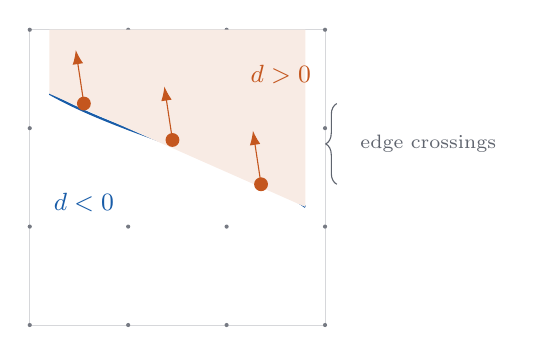
\begin{tikzpicture}[scale=1.25]
  \draw[grid] (0,0) rectangle (3,3);
  \foreach \x in {0,1,2,3} \foreach \y in {0,1,2,3}
    \fill[ink!60] (\x,\y) circle (0.6pt);
  % a slice
  \draw[accent,thick] (0.2,2.35) .. controls (1.0,1.9) and (2.1,1.7) .. (2.8,1.2);
  \fill[accent2!12] (0.2,2.35) -- (2.8,1.2) -- (2.8,3) -- (0.2,3) -- cycle;
  % crossings and normals
  \foreach \x/\y/\nx/\ny in {0.55/2.25/-0.15/0.99, 1.45/1.88/-0.15/0.99, 2.35/1.43/-0.15/0.99} {
    \fill[accent2] (\x,\y) circle (2pt);
    \draw[accent2,-{Latex[length=1.8mm]}] (\x,\y) -- ++(\nx*0.55,\ny*0.55);
  }
  \node[accent2,font=\small] at (2.55,2.55) {$d>0$};
  \node[accent,font=\small] at (0.55,1.25) {$d<0$};
  \draw[decorate,decoration={brace,amplitude=4pt},ink!70]
    (3.12,1.43) -- (3.12,2.25) node[midway,right=5pt,font=\scriptsize]{edge crossings};
\end{tikzpicture}
\caption{A surface cell in two dimensions.  The shaded region is the
inside ($d<0$).  Sign changes on cube edges give crossing points and
normals; the QEF fits a dual vertex to those planes.  In three dimensions
there are twelve cube edges, and the vertex is clamped inside the cube.}
\label{fig:qef2d}
\end{figure}

\subsection{Brushes, painters, and mapping state}

The node stores the brush index, an HSV tint, the texture-mapping mode, and
two generic data values.  The brush is painted at the shape leaf; internal
nodes inherit the dominant painted child.  The GPU vertex payload packs:
\begin{center}
\begin{tabular}{@{}lll@{}}
\toprule
Word & Components & Source\\
\midrule
0 & position.xyz, color.x & QEF position; color is 1\\
1 & color.yz, texCoord.xy & texCoord = node data (UV scale)\\
2 & normal.xyz, brushIndex bits & normalized SDF gradient; brush\\
3 & textureType bits, hsv & mapping mode; HSV tint\\
\bottomrule
\end{tabular}
\end{center}
The renderer treats the 64-byte record as the canonical \code{Vertex}; the
same record is used by the raster path, the ray-tracing BLAS, and the
offline exporter.  This is why the finalize stage does not need a
conversion pass.

\section{The CPU octree data structure}
\label{sec:octreedata}

\subsection{Node layout}

An \code{OctreeNode} is a compact record:
\begin{center}
\begin{tabular}{@{}p{0.32\linewidth}p{0.60\linewidth}@{}}
\toprule
Field & Purpose\\
\midrule
\code{float sdf[8]} & eight corner samples (may contain $+\infty$)\\
\code{int brushIndex} & material index, or the discard sentinel\\
\code{int textureType} & triplanar / projection / custom mapping\\
\code{glm::vec2 data} & mapping scale or authored UV\\
\code{glm::vec3 hsv} & tint carried to the vertex payload\\
\code{uint8_t lod} & stored ladder level, +1 shifted; $0$ = unset\\
\code{uint8_t chunkLod} & chunk-rung level, +1 shifted; $0$ = not a chunk\\
\code{uint8_t bits} & leaf flag, chunk flag, type\\
\code{uint blockId} & index of the child block in the allocator\\
\code{uint version} & bump on every published revision\\
\bottomrule
\end{tabular}
\end{center}

The +1 shift is a storage trick: a single byte can represent ``unset''
(0) and levels 0--254 without a separate sentinel.  Every propagator uses
the same convention:
\begin{equation}
  lod_{\text{parent}} = \min_i lod_{\text{child},i} + 1,
  \qquad
  chunkLod_{\text{parent}} = \min_i chunkLod_{\text{child},i} + 1 .
\end{equation}
The GPU shader compares the stored level directly against the target
level; no shift is applied in the shader.

Children are stored in a separate \code{ChildBlock}, an eight-entry array
allocated from an \code{OctreeAllocator}.  A leaf has no block; an internal
node has a block with up to eight children.  The allocator is a pool of
blocks and nodes; freeing a subtree returns blocks to the pool and bumps
the generation of the parent.  Because node addresses are recycled, every
publish/delete handler must be paired: a new node at a recycled address
must not inherit the previous occupant's pending mesh.  The engine's
change handler explicitly reports the whole deleted subtree before
\code{clear()} releases the children.

\subsection{Cube corners and edges}

The corner convention is bit-based:
\begin{center}
\begin{tabular}{@{}c|ccc@{}}
\toprule
$i$ & $x$ & $y$ & $z$\\
\midrule
0 & 0 & 0 & 0\\
1 & 0 & 0 & 1\\
2 & 0 & 1 & 0\\
3 & 0 & 1 & 1\\
4 & 1 & 0 & 0\\
5 & 1 & 0 & 1\\
6 & 1 & 1 & 0\\
7 & 1 & 1 & 1\\
\bottomrule
\end{tabular}
\end{center}
The twelve edges are
\begin{equation}
\begin{aligned}
&(0,1),(1,3),(2,3),(0,2),\\
&(4,5),(5,7),(6,7),(4,6),\\
&(0,4),(1,5),(2,6),(3,7).
\end{aligned}
\label{eq:edges}
\end{equation}
This ordering is load-bearing: the QEF loop, the GPU scan loop, the
Blender exporter, and the CPU reference all iterate the same twelve edges
in the same order.  Changing it changes the floating-point accumulation
order and therefore the last bits of a vertex position.

\begin{figure}[htbp]
\centering
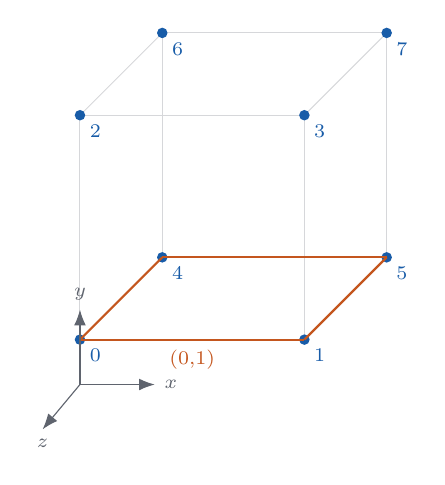
\begin{tikzpicture}[scale=0.95]
  % back face
  \draw[grid] (0,0) rectangle (3,3);
  % front face offset
  \draw[grid] (1.1,1.1) rectangle (4.1,4.1);
  \foreach \p in {(0,0),(3,0),(0,3),(3,3)} \draw[grid] \p -- ++(1.1,1.1);
  % corners
  \foreach \x/\y/\lab in {0/0/0,3/0/1,0/3/2,3/3/3,1.1/1.1/4,4.1/1.1/5,1.1/4.1/6,4.1/4.1/7}
    \fill[accent] (\x,\y) circle (2pt) node[below right,font=\scriptsize]{\lab};
  % edges highlighted
  \draw[accent2,thick] (0,0)--(3,0) node[midway,below,font=\scriptsize]{(0,1)};
  \draw[accent2,thick] (3,0)--(4.1,1.1);
  \draw[accent2,thick] (0,0)--(1.1,1.1);
  \draw[accent2,thick] (1.1,1.1)--(4.1,1.1);
  % axes
  \draw[-{Latex[length=2mm]},ink!70] (0,-0.6)--(1,-0.6) node[right,font=\scriptsize]{$x$};
  \draw[-{Latex[length=2mm]},ink!70] (0,-0.6)--(0,0.4) node[above,font=\scriptsize]{$y$};
  \draw[-{Latex[length=2mm]},ink!70] (0,-0.6)--(-0.5,-1.2) node[below,font=\scriptsize]{$z$};
\end{tikzpicture}
\caption{Corner numbering and the first four edges.  The cube is drawn with
$z$ receding; the corner bits are $(x,y,z)$ with bit 2 $=x$, bit 1 $=y$,
bit 0 $=z$.  The GPU table stores corners in two \code{vec4}s and edges as
twelve integer pairs.}
\label{fig:corners}
\end{figure}

\subsection{Types and sentinels}

Each node has a \code{SpaceType}: \code{Empty}, \code{Surface}, or
\code{Solid}.  The classification uses \code{SDF::eval}:
\begin{equation}
  \operatorname{eval}(\mathbf{d}) =
  \begin{cases}
    \text{Empty}, & \text{no finite negative corner and no finite positive corner},\\
    \text{Solid}, & \text{all finite corners negative},\\
    \text{Surface}, & \text{otherwise (both signs present)}.
  \end{cases}
\end{equation}
An all-$+\infty$ cell is Empty.  A cell with only positive finite corners
is Empty.  A cell with only negative finite corners is Solid.  A cell with
both is Surface.  The edge scan is stricter: it tests the \emph{sign pair}
of each edge directly, so a surface cell whose only negative corner is
diagonally opposite a positive one may have no active cube edge; the scan
simply emits nothing.

\subsection{Level of detail and chunk ladder}

Two distinct levels live on a node:
\begin{description}
\item[\code{lod}] the simplification ladder level.  A leaf at the
  tessellation frontier has $lod=1$; a parent whose eight children can be
  collapsed has $lod=\min child + 1$; the root has the largest value.
\item[\code{chunkLod}] the chunk rung.  A node is a chunk root when its
  cube is between $\Delta/2$ and $\Delta$; its immediate descendants are
  marked $chunkLod=1$, their children $2$, and so on.  The renderer's LoD
  gate consumes this value.
\end{description}
The chunk size $\Delta$ is fixed per scene (for example $512$ world
units).  A chunk root at level 0 is the finest published rung; its
ancestors form the coarser rungs.  The renderer keeps exactly one rung per
region visible, which is why the mesher publishes every rung rather than
only the finest one.

\begin{figure}[htbp]
\centering
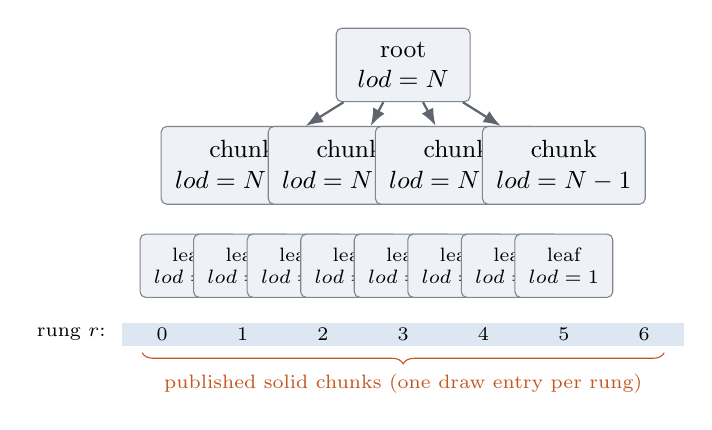
\begin{tikzpicture}[scale=0.85]
  % tree
  \node[box,minimum width=17mm] (root) at (0,3.2) {root\\$lod=N$};
  \foreach \i/\x in {0/-2.4,1/-0.8,2/0.8,3/2.4} {
    \node[box,minimum width=14mm] (c\i) at (\x,1.7) {chunk\\$lod=N-1$};
    \draw[arrow] (root) -- (c\i);
  }
  \foreach \i/\x in {0/-3.2,1/-2.4,2/-1.6,3/-0.8,4/0.0,5/0.8,6/1.6,7/2.4} {
    \node[box,minimum width=11mm,font=\scriptsize] (g\i) at (\x,0.2) {leaf\\$lod=1$};
  }
  % ladder bar
  \fill[accent!15] (-4.2,-1.0) rectangle (4.2,-0.65);
  \foreach \x/\t in {-3.6/0,-2.4/1,-1.2/2,0/3,1.2/4,2.4/5,3.6/6}
    \node[font=\scriptsize] at (\x,-0.82) {\t};
  \node[font=\scriptsize,left] at (-4.3,-0.82) {rung $r$:};
  \draw[decorate,decoration={brace,mirror,amplitude=4pt},accent2]
    (-3.9,-1.1) -- (3.9,-1.1) node[midway,below=4pt,font=\scriptsize]{published solid chunks (one draw entry per rung)};
\end{tikzpicture}
\caption{The chunk ladder.  Every surface-bearing cell whose size lies in
$(\Delta/2,\Delta]$ is a chunk root at some rung.  Its children are the
next finer rung, and so on.  The GPU gate walks this dyadic lattice from
the root to choose exactly one visible rung per region.}
\label{fig:ladder}
\end{figure}

\subsection{Memory model}

The octree is a sparse pointer structure, not a dense grid.  A node is
small (the eight floats dominate) and a block is eight pointers.  For a
reference terrain with about $10^6$ surface cells the node storage is on
the order of tens of megabytes, which is small compared with the GPU
pools.  The expensive part is not the octree itself but the per-chunk
flattened upload: a chunk's neighbourhood can contain several thousand
nodes, each uploaded as a 128-byte record (eight floats, cube, metadata,
HSV/mapping, children).  \Cref{sec:perf} measures this traffic.

\subsection{Concurrency}

\code{Octree::apply} takes a unique lock on \code{treeMutex}; every
iteration (`iterateMultiThreaded`, the exporter walk, the debug cube walk)
takes a shared lock.  The shape recursion forks at a band of cube sizes and
joins its children before returning, so a tree never exposes a partially
written child block to a reader.  The flattening runs under the shared
lock: it reads the tree structure and copies the neighbourhood into a
private \code{OctreeTopologyInput}.  The GPU pass then works on the copy,
so the tree can be edited again while the GPU is still meshing an older
snapshot.  The version recorded in the chunk manager (not the pointer)
decides whether a rebuild is needed.

\section{CPU shape construction: \code{Octree::apply}}
\label{sec:cpushape}

\subsection{Entry point and root expansion}

An edit is expressed as
\begin{lstlisting}[caption={The public shape entry point (simplified).},label={lst:apply}]
void Octree::apply(operation, function, model, painter, coordPainter,
                   minSize, simplifier, updateHandler, deleteHandler) {
    unique_lock treeLock(treeMutex);
    ShapeArgs args = ...;       // operation, function, model, painter, simplifier
    expand(args);               // grow the root if the new shape lies outside
    configureShapeCache(args);  // lattice origin/spacing for this apply
    OctreeNodeFrame frame(root, nullptr, *this, ...);
    NodeOperationResult r;
    shape(r, frame, args, &localContext, updateHandler, deleteHandler);
}
\end{lstlisting}

\code{expand} grows the root by powers of two until the new primitive is
fully contained.  It computes the child index of the primitive's centre in
the current root cube and places the old root as that child of a new,
doubled root.  This is the only operation that changes the world cube; the
existing subtree is preserved bit-for-bit.  The lattice origin and leaf
length used by the SDF cache are computed \emph{after} expansion.

\subsection{The recursive \code{shape} call}

For a cube of length $L$ and a target leaf size $m$, the recursion has
three regimes:
\begin{enumerate}
\item \textbf{Leaf:} $L\le m$ and the node is a leaf.  Sample the eight
  corners of the shape field, combine them with the existing field, and
  classify the result.
\item \textbf{Interior with early out:} the node is not a leaf, but the
  shape field's centre value and bounding-volume test prove that the
  primitive cannot affect this cube.  Copy the existing field and stop.
\item \textbf{Interior descend:} recurse into the eight children, join the
  results, classify the parent from the children, and optionally simplify.
\end{enumerate}

\begin{figure}[htbp]
\centering
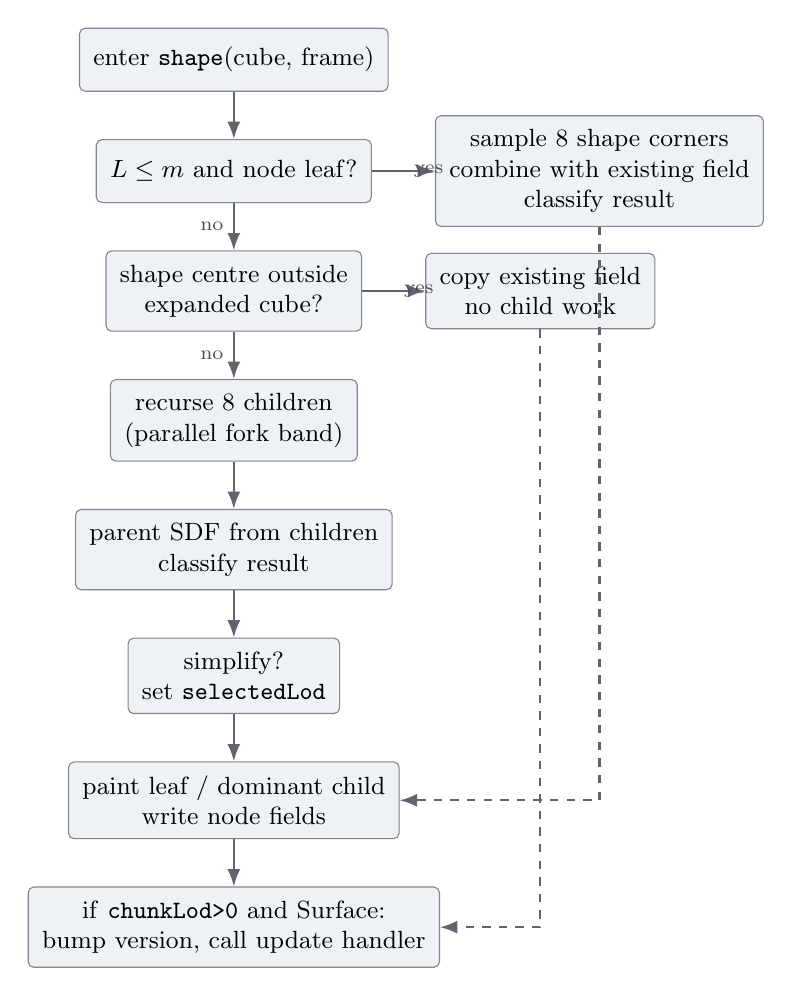
\begin{tikzpicture}[node distance=6mm and 8mm,font=\small]
  \node[box] (enter) {enter \code{shape}(cube, frame)};
  \node[box,below=of enter] (leaf) {$L\le m$ and node leaf?};
  \node[box,right=of leaf] (sample) {sample 8 shape corners\\combine with existing field\\classify result};
  \node[box,below=of leaf] (outside) {shape centre outside\\expanded cube?};
  \node[box,right=of outside] (copy) {copy existing field\\no child work};
  \node[box,below=of outside] (children) {recurse 8 children\\(parallel fork band)};
  \node[box,below=of children] (parent) {parent SDF from children\\classify result};
  \node[box,below=of parent] (simp) {simplify?\\set \code{selectedLod}};
  \node[box,below=of simp] (paint) {paint leaf / dominant child\\write node fields};
  \node[box,below=of paint] (publish) {if \code{chunkLod>0} and Surface:\\bump version, call update handler};
  \draw[arrow] (enter)--(leaf);
  \draw[arrow] (leaf)--node[right,note]{yes}(sample);
  \draw[arrow] (leaf)--node[left,note]{no}(outside);
  \draw[arrow] (outside)--node[right,note]{yes}(copy);
  \draw[arrow] (outside)--node[left,note]{no}(children);
  \draw[arrow] (children)--(parent);
  \draw[arrow] (parent)--(simp);
  \draw[arrow] (simp)--(paint);
  \draw[arrow] (paint)--(publish);
  \draw[arrow,dashed] (sample) |- (paint);
  \draw[arrow,dashed] (copy) |- (publish);
\end{tikzpicture}
\caption{The shape recursion.  A leaf samples the new field; an unaffected
interior copies the old field; an affected interior recurses, classifies
the parent from its children, simplifies, paints, and (for surface chunk
roots) publishes a new version.}
\label{fig:shapeflow}
\end{figure}

\subsection{Sampling and caching}

The shape field is sampled at cube corners with \code{evaluateSDF}.  A
naive implementation calls the primitive's distance function once per
query.  The engine uses a per-apply cache keyed on the apply's leaf lattice:
\begin{equation}
  \mathbf{x} = \mathbf{o} + \mathbf{n}\,h,
\end{equation}
where $\mathbf{o}$ is the lattice origin and $h$ the half leaf length.
An integer lattice key is accepted only when the reconstructed float is
bit-identical to the query.  Anything off-lattice (a stored tree from an
earlier apply with a smaller leaf size) falls back to a float-keyed map.
The cache is a pure optimisation: the returned value is the value the
primitive would produce.  The cache is per-thread, generation-tagged, and
reset when the generation changes.  This avoids both a global lock and
stale values across applies.

\subsection{The three early-out rules}

The recursion has three important early outs.  They are necessary for
performance and for correctness at the field's infinity regions.

\paragraph{All-infinity node.}
If no corner of the existing field has data, the node is untouched.  The
operation may propagate from infinity (a union with a finite shape) or not
(a subtraction whose negative operand is undefined).  If the shape's
centre is more than the cube's half-diagonal away from the solid, the
whole cube is classified Solid or Empty without descending.

\paragraph{Solid-preserving operation.}
If the existing cube is Solid, all its corners finite, and the operation
preserves solidity, the result is still Solid.  The operation only needs
to combine the existing and shape corner values; no child descent is
needed.  This is the common case for a union of overlapping solids.

\paragraph{Solid cube and centre test.}
If the existing cube is Solid and the combined centre is more than the
cube's half-diagonal inside the surface, the whole cube is Solid.  This
avoids descending into regions the new shape cannot reach.  The test uses
the half diagonal $L\sqrt{3}/2$, not the half edge: a sphere can enter
through a corner.

If none of the early outs applies, the function's \code{check(cube)} test
is consulted.  A \code{Disjoint} result skips the children; a
\code{Contains} result can be handled by the same solid/empty rules.
Finally, if the node is a new surface node with no existing children, the
recursion is forced to descend even if the centre is outside, because the
surface may still cross a corner.

\subsection{Result composition}

For a non-leaf node, each child returns eight result SDF values.  The
parent's result array is the concatenation of the children's corner arrays
in child order.  The parent's type is:
\begin{equation}
  \operatorname{parentType} =
  \begin{cases}
    \text{Empty}, & \text{all children Empty},\\
    \text{Solid}, & \text{all children Solid},\\
    \text{Surface}, & \text{otherwise}.
  \end{cases}
\end{equation}
This is exact because the child corner arrays share the parent's corners
on their common faces.  The parent does not need to re-evaluate the field.

\subsection{Painting}

Painting happens at the shape leaf, where the node's material is decided.
Brushes can be constant (a material index), procedural (terrain
classification from height and slope), or position-dependent (the
\code{LandBrush} classifier).  The painter writes:
\begin{itemize}
\item \code{brushIndex} (material),
\item \code{hsv} (tint),
\item \code{textureType} (mapping technique),
\item \code{data} (UV scale or authored UV).
\end{itemize}
Internal nodes inherit the dominant painted child's state.  The exact
dominance rule is intentionally simple: the last surface child with a
valid brush that wins the per-child tally sets the parent.  The tally is
kept per child (not across all eight) so the historical result is
preserved; changing it would change the mesh's material assignment and UV
scale.

\subsection{Node publishing and versions}

A node that is both a surface and a chunk root (\code{chunkLod>0}) is a
published chunk.  At the end of its recursion, the engine:
\begin{enumerate}
\item sets its type, SDF, chunk flag, levels, brush, mapping state;
\item increments \code{version};
\item calls the update handler with \code{(level, node, cube)}.
\end{enumerate}
The handler queues a \code{PendingMeshData}.  The renderer later flattens
the neighbourhood, dispatches the GPU walk, and publishes the span.  A
version is the only identity the renderer trusts: the same node address may
be reused by the allocator, so pointer identity alone is not a revision.

\subsection{Threading}

The recursion forks when the child cube length lies in
\begin{equation}
  \left(\frac{m\cdot 16}{4},\;m\cdot 16\right],
\end{equation}
where $m$ is the target leaf size.  A forked node enqueues eight tasks into
the octree's thread pool; each task owns a copy of its frame and the shape
arguments and writes into a shared result block.  The parent joins all
eight futures before reading the block.  The fork band is two levels deep:
a $16m$ node forks eight $8m$ children and each of those forks eight $4m$
grandchildren; the $4m$ nodes do not fork again.  This bounds the number of
tasks per fork to 64 and avoids a thundering herd at the leaf level.

The join loop is careful about pool starvation.  Instead of blocking on a
future while the pool is idle, it calls \code{runOneTask()} to execute
queued work on the waiting thread; only when the queue is empty does it
block.  This is what keeps a nested fork from deadlocking on a pool with
fewer threads than the fan-out.

\subsection{Why the CPU never solves a vertex}

The current shape path deliberately avoids \code{SDF::getPosition} and
\code{getNormalFromPosition}.  The only host callers are the offline
Blender exporter.  This is not just a performance choice: it is a
correctness boundary.  If the runtime computed a vertex on the host and the
GPU computed another, the two would differ in the last bits and the
renderer's mesh would not match the exporter's.  By making the GPU the sole
Cartesian producer, the runtime has one answer and the exporter has a
reference implementation that can be compared offline.

\section{Simplification and the LoD ladder}
\label{sec:lod}

\subsection{What simplification means here}

The octree's leaf lattice is the finest representation the shape pass ever
produces.  A coarser representation is obtained by removing all children of
a node and treating its eight interpolated corners as the node's SDF.  The
node then becomes a leaf at a coarser level and its dual vertex is solved
from the coarser eight samples.  The mesh is still a valid dual mesh; it
simply has fewer, larger cells.

Simplification is not a decimation of an existing triangle mesh.  It is a
decision made during the shape recursion, before any triangle exists.  This
is why the GPU can rebuild a chunk at any rung without a separate
simplification pass: the tree already stores the chosen level.

\subsection{The error criterion}

For a candidate parent cube and its eight child results, the simplifier
tests each surface child.  For every corner of the child cube it computes
the parent field's trilinear value and compares it with the child's stored
corner value:
\begin{equation}
  e = \max_{i\in\text{surface children}}\;
      \max_{j=0}^{7}
      \left| \operatorname{interp}(\mathbf{d}_{\text{parent}},
      C_{i,j}) - d_{i,j} \right|.
\end{equation}
The parent may collapse only when $e \le \tau L$, where $L$ is the parent
edge and $\tau$ a user tolerance.  A flat surface has small error and
collapses; a cliff, a thin wall, or a sharp CSG seam has large error and
stays subdivided.

\begin{lstlisting}[caption={The simplifier's core checks (abridged).},label={lst:simplify}]
SimplificationResult Simplifier::simplify(cube, sdf, children, chunkCube) {
    // 1. material consistency (texturing mode):
    //    all surface children must share one brush and be leaves
    // 2. chunk-border guard:
    //    never simplify a direct child of a chunk root
    // 3. re-interpolation error:
    //    for each surface child corner, |parent interp - child value|
    //    must be <= cube.getLengthX() * distance
    return result;
}
\end{lstlisting}

\subsection{The material and chain guards}

Two non-geometric guards are essential:

\begin{enumerate}
\item \textbf{Material boundary.}  If two surface children have different
  brushes, collapsing them would force one material onto the other.  The
  simplifier refuses.  This keeps a grass/rock boundary sharp even when the
  geometric error is small.
\item \textbf{Simplification chain.}  A child may be collapsed only if it is
  itself a leaf.  If a child still has children, collapsing the parent
  would skip a level of the ladder and break the hierarchy's monotonicity.
\end{enumerate}

\subsection{The chunk-border guard}

A chunk root's direct children have length $\Delta/2$.  They are the
boundary cells between two chunks.  If one chunk simplified such a cell and
its neighbour did not, the two dual meshes would choose different edge
vertices at the same boundary.  The stitching algorithm can handle
different cell sizes in the \emph{interior} of the adaptive walk, but the
chunk boundary is special: the two chunks are flattened independently and
never share a node table.  The guard therefore forbids simplifying the
direct children of a chunk root.  Coarser simplification is allowed only
deeper in the subtree, where both sides of a boundary see the same
neighbourhood and the break collector can stitch.

\subsection{Level propagation}

Each node's stored level is the minimum over its surface children plus one:
\begin{equation}
  lod(v) =
  \begin{cases}
    1, & v \text{ is a leaf at the frontier},\\
    0, & v \text{ is not a surface node},\\
    \min_{c\in\text{children}(v)} lod(c) + 1, & \text{otherwise}.
  \end{cases}
\end{equation}
The renderer uses the level as the rung index.  The chunk's own level is
propagated the same way but only along the chunk ladder:
\begin{equation}
  chunkLod(v) =
  \begin{cases}
    1, & v \text{ is a chunk root},\\
    \min_{c} chunkLod(c)+1, & \text{otherwise}.
  \end{cases}
\end{equation}
The published entry stores the 0-based \code{lod} (the shader/indirect gate
subtracts one implicitly).  A node with \code{chunkLod>0} and
\code{resultType==Surface} gets a version bump and is published.

\subsection{Why every rung is published}

It is tempting to publish only the finest rung and let the renderer collapse
it.  That fails for two reasons:

\begin{itemize}
\item \textbf{The tree is sparse.}  A coarse region may have no fine leaf at
  all; the only representation is the coarse node's eight samples.
\item \textbf{The dual mesh is not a simple triangle subset.}  A coarse cell
  produces a different dual vertex and a different ring than its eight
  fine children.  Decimating the fine mesh is not equivalent to solving the
  coarse dual mesh.
\end{itemize}

Publishing every rung gives the GPU gate a complete ladder.  The gate then
selects exactly one rung per region, so the extra rungs cost memory but not
draw calls.  The memory is bounded by the number of chunk-bearing nodes
(about one per $(\Delta/2,\Delta]$ cell) and is preallocated.

\subsection{Chunk versions and rebuilds}

Every published chunk carries a version.  The scene layer records the
version it has already emitted; a publish with the same version is
\code{UpToDate} and is skipped.  An edit bumps the version of the affected
chunk roots and their ancestors.  The renderer's pending queue then
contains a new entry for each affected rung.  The old span remains in the
pool until the new span is published, so no frame ever sees a hole.

\subsection{Cost model}

Let $C$ be the number of surface cells at the finest lattice, $N$ the
number of nodes in the tree, and $R$ the number of ladder rungs.  The
simplifier is linear in the number of surface children and corner tests:
\begin{equation}
  T_{\text{simplify}} = \Oh(N R \, 8 \cdot 8)
\end{equation}
in the worst case, but in practice most nodes fail the first material or
chain guard and do not reach the corner loop.  The dominant cost of a
shape apply is the field evaluation, not the simplifier.  The cache makes
repeated corner evaluations across neighbouring cubes cheap.

\section{The CPU reference walker}
\label{sec:cpuwalk}

The CPU walker is \code{OctreeTriangleTessellator::iterateTriangles}.  It is
no longer used at runtime, but it defines the semantics the GPU shader must
reproduce and it is the only mesher used by the offline Blender exporter.
Reading it is the best way to understand the GPU port because the shader is
a line-by-line translation with an explicit stack instead of C++
recursion.

\subsection{Frontier and scan cells}

The walk starts at a chunk node and a target LoD $r$.  It descends to the
cells at that rung:
\begin{lstlisting}[caption={Frontier descent (conceptual).},label={lst:frontier}]
void walk(node, cube, targetLod) {
    if (node.lod == targetLod) {
        scanCell(node, cube);
    } else if (node.lod > targetLod) {
        for (child in node.children) walk(child, cube.child(i), targetLod);
    }
}
\end{lstlisting}
A \emph{scan cell} is a cube at the target rung.  Only cells that straddle
the surface need to be scanned.  The GPU flattening compacts the list with
the same ``has negative and non-negative corner'' test, because a cell with
no sign change on any of its twelve edges cannot emit a triangle.

\subsection{Twelve edges and edge spans}

For a scan cell with cube minimum $\mathbf{c}$ and size $L$, each of the
twelve edges is converted to an \code{EdgeSpan}:
\begin{itemize}
\item \code{axis}: the edge's varying axis (the one with the largest
  coordinate difference, which is exact for an axis-aligned cube);
\item \code{fixedU}, \code{fixedV}: the two constant coordinates;
\item \code{start}, \code{end}: the varying coordinate interval;
\item \code{eps}: the geometric epsilon
  $\max(\text{worldSize}, L)\cdot 10^{-6}$;
\item \code{sampleOffset}: $L\cdot10^{-3}$, used to nudge boundary samples.
\end{itemize}
The span is active only when its two corner SDF values have opposite signs.
The sign of the endpoint is also remembered; it is the authoritative
winding oracle.

\subsection{Why one edge can produce many segments}

In a uniform grid, an active edge is shared by exactly four cells, all of
the same size.  The dual polygon is a quad (or a triangle when one of the
four cells is not a surface cell).  In an adaptive octree, the four
quadrant cells around an edge can have different sizes and can be nested.
The edge can cross several cell boundaries along its length.  The correct
mesh must split the edge at every such boundary; otherwise one side of the
boundary would connect to a vertex that the other side does not know.

\begin{figure}[htbp]
\centering
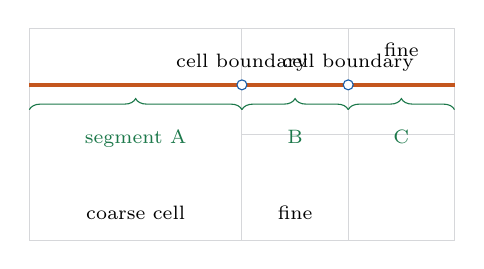
\begin{tikzpicture}[scale=0.9]
  % coarse cell left, fine right
  \draw[grid] (0,0) rectangle (3,3);
  \draw[grid] (3,0) rectangle (6,3);
  \draw[grid] (3,1.5) -- (6,1.5);
  \draw[grid] (4.5,0) -- (4.5,1.5);
  \draw[grid] (4.5,1.5) -- (4.5,3);
  % edge
  \draw[accent2,line width=1.2pt] (0,2.2) -- (6,2.2);
  % cell boundary crossings
  \foreach \x/\lab in {3.0/coarse|fine, 4.5/fine|fine} {
    \draw[accent,fill=white] (\x,2.2) circle (2pt);
  }
  \node[font=\scriptsize,above] at (3,2.25) {cell boundary};
  \node[font=\scriptsize,above] at (4.5,2.25) {cell boundary};
  % subsegments
  \draw[decorate,decoration={brace,amplitude=4pt},good]
    (0,1.85) -- (3,1.85) node[midway,below=4pt,font=\scriptsize]{segment A};
  \draw[decorate,decoration={brace,amplitude=4pt},good]
    (3,1.85) -- (4.5,1.85) node[midway,below=4pt,font=\scriptsize]{B};
  \draw[decorate,decoration={brace,amplitude=4pt},good]
    (4.5,1.85) -- (6,1.85) node[midway,below=4pt,font=\scriptsize]{C};
  % cell labels
  \node[font=\scriptsize] at (1.5,0.4) {coarse cell};
  \node[font=\scriptsize] at (3.75,0.4) {fine};
  \node[font=\scriptsize] at (5.25,2.7) {fine};
\end{tikzpicture}
\caption{An active edge crossing a coarse/fine cell boundary.  The edge is
split at every cell boundary coordinate; each sub-segment is emitted by its
owner cell.  Both the coarse and the fine side collect the same set of
boundaries, so the resulting rings agree along the shared edge.}
\label{fig:edge-split}
\end{figure}

\subsection{Collecting breaks}

The break collector is the heart of the adaptive stitching.  Given an edge
span and an interval $[a,b]$, it samples the four quadrant cells at the
midpoint.  Each valid cell contributes its cube's minimum and maximum
coordinate along the edge axis.  If these coordinates lie strictly inside
$[a,b]$, they become breakpoints.  The interval is then recursively split
at each breakpoint and the process repeats.  The recursion stops when the
interval is shorter than $2\epsilon$ or contains no new break.

The crucial detail is that the four quadrant cells are resolved by
\code{findCellAt}, a root-to-cell descent that mirrors the octree's
\code{getChildIndex} arithmetic.  A sample is nudged by one ulp in the two
fixed axes so that a point exactly on a cell face does not land in both
cells; a small normal offset replaces the ulp when the value is zero (the
next float is subnormal and may be flushed to zero).  The four samples are:
\begin{align}
  (\text{fixedU}-\delta,\;& \text{fixedV}-\delta),\\
  (\text{fixedU}+\delta,\;& \text{fixedV}-\delta),\\
  (\text{fixedU}-\delta,\;& \text{fixedV}+\delta),\\
  (\text{fixedU}+\delta,\;& \text{fixedV}+\delta).
\end{align}
The first sample is resolved with a full descent; the other three reuse it
if they still lie inside its cube, which is exact because \code{findCellAt}
is a pure function of position.  This is the same optimization in the CPU
walker and the shader.

\subsection{The break list and the interval stack}

The CPU collector uses recursive calls and a \code{std::vector<float>}
break list.  The GPU port replaces recursion with an explicit LIFO stack:
\begin{lstlisting}[style=glsl,caption={The GPU break collector (shape).},label={lst:breaks}]
void collectBreaks(edge, start, end) {
    pushTask(start, end);
    while (top > 0) {
        pop(a, b);
        if (b - a <= eps*2) continue;
        mid = 0.5*(a+b);
        local = {a,b};
        cells = sampleQuadrants(edge, mid);
        for each valid cell:
            addBreakLocal(cell.min[axis], a, b);
            addBreakLocal(cell.min[axis]+cell.size, a, b);
        sortUniqueLocal();
        for interior local breaks: addBreakGlobal(...);
        push sub-intervals in reverse order;
    }
}
\end{lstlisting}
The CPU version appends all interior breaks before recursing into the
sub-intervals.  The GPU version reproduces that order by pushing the
sub-intervals in reverse so the LIFO pop visits them left to right.  The
global break list is therefore identical up to floating-point ordering.

The fixed capacities are part of the contract:
\begin{center}
\begin{tabular}{@{}lll@{}}
\toprule
Buffer & Capacity & Meaning\\
\midrule
\code{BREAK\_CAP} & 64 & final breaks per edge span\\
\code{LOCAL\_BREAK\_CAP} & 32 & breaks inside one interval\\
\code{TASK\_STACK} & 256 & pending intervals\\
\code{POS\_MEMO} & 8 & QEF position cache per invocation\\
\bottomrule
\end{tabular}
\end{center}
A cap overflow does not truncate silently.  \code{noteOverflow()} sets a
per-invocation flag and increments \code{overflowCount}; the host fails the
chunk and retries it instead of drawing a hole.

\subsection{Owner selection}

For each sub-segment $[a,b]$, the owner is the surface quadrant with the
smallest ordering key:
\begin{enumerate}
\item smaller cube size first;
\item then smaller $x$ minimum;
\item then smaller $y$ minimum;
\item then smaller $z$ minimum;
\item then smaller node index (a deterministic stand-in for pointer order).
\end{enumerate}
The owner is computed from the four quadrants at the segment midpoint, not
from the scan cell.  This is what makes two neighbouring chunks agree: both
see the same four quadrant cells and both choose the same owner.

\subsection{Polygon reconstruction}

The four quadrants are filtered to surface cells and deduplicated by node
identity and by position (within the edge epsilon).  A coarse ancestor can
appear in two opposite quadrants of the ring; the old code only removed
adjacent duplicates and then rejected the whole segment, which produced
the missing surface along the world axes.  The current code deduplicates
against every already-collected quadrant.  If the resulting list has three
or four entries, it is rotated so the owner is first; then it is fanned into
one or two triangles.

\begin{figure}[htbp]
\centering
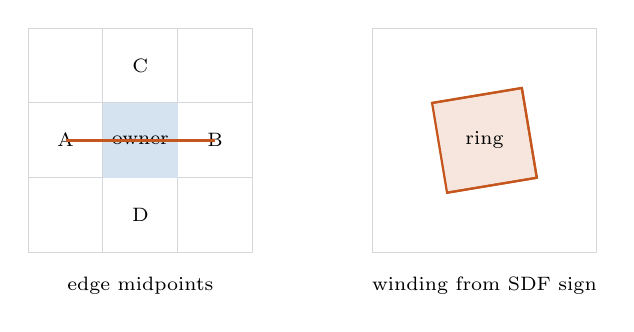
\begin{tikzpicture}[scale=0.95]
  \begin{scope}[shift={(0,0)}]
    \draw[grid] (0,0) rectangle (3,3);
    \draw[grid] (1,0)--(1,3); \draw[grid] (2,0)--(2,3);
    \draw[grid] (0,1)--(3,1); \draw[grid] (0,2)--(3,2);
    \fill[accent!18] (1,1)--(2,1)--(2,2)--(1,2)--cycle;
    \node[font=\scriptsize] at (1.5,1.5) {owner};
    \node[font=\scriptsize] at (0.5,1.5) {A};
    \node[font=\scriptsize] at (2.5,1.5) {B};
    \node[font=\scriptsize] at (1.5,2.5) {C};
    \node[font=\scriptsize] at (1.5,0.5) {D};
    \draw[accent2,line width=1pt] (0.5,1.5)--(1.5,1.5)--(2.5,1.5);
    \node[below,font=\scriptsize] at (1.5,-0.2) {edge midpoints};
  \end{scope}
  \begin{scope}[shift={(4.6,0)}]
    \draw[grid] (0,0) rectangle (3,3);
    \draw[accent2,fill=accent2!15] (1.0,0.8)--(2.2,1.0)--(2.0,2.2)--(0.8,2.0)--cycle;
    \draw[accent2,thick] (1.0,0.8)--(2.2,1.0)--(2.0,2.2)--(0.8,2.0)--cycle;
    \node[font=\scriptsize] at (1.5,1.5) {ring};
    \draw[accent2,thick] (0.8,2.0)--(2.0,2.2);
    \draw[accent2,thick] (2.0,2.2)--(2.2,1.0);
    \draw[accent2,thick] (2.2,1.0)--(1.0,0.8);
    \node[below,font=\scriptsize] at (1.5,-0.2) {winding from SDF sign};
  \end{scope}
\end{tikzpicture}
\caption{Left: the four quadrant cells around an edge.  Right: the dual
polygon is the ring of their vertices.  The ring is rotated so the owner
leads, then fanned.  The winding is chosen from the SDF sign at the edge
start, not from the normals.}
\label{fig:ring}
\end{figure}

\subsection{Winding}

The triangle order must be consistent with the SDF sign.  The walker takes
the interpolated SDF at the segment start using the owner's field.  If the
owner's interpolation is infinite or degenerates, it falls back to the
producing cell's endpoint sign.  A solid start means the ring is ordered
so the outward normal points away from the solid; a positive start means
the order is reversed.  The sign is an \emph{authoritative oracle}: it is
independent of the QEF normal, which can degrade at coarse levels and on
non-planar quads.  This is why the surface does not flip at LoD
transitions.

\subsection{Triangle fan and duplicate rejection}

A 3-ring produces one triangle; a 4-ring produces two, fanned around the
owner.  Before emission, the three dual positions are compared; if any two
are within the edge epsilon, the triangle is dropped.  A degenerate QEF
vertex (or two cells that collapsed to the same position) must not create a
zero-area triangle: it would break normals, shadows, and ray tracing.

\subsection{The CPU triangle handler}

The CPU walker passes each triangle to \code{Tesselator::handle}, which:
\begin{itemize}
\item resolves the three cell vertices to \code{Vertex} records;
\item copies brush, HSV, texture type, and mapping data;
\item computes the triplanar UV plane from the face normal;
\item appends the triangle to the chunk's \code{Geometry}.
\end{itemize}
The GPU port does not have a \code{Tesselator} equivalent.  Stage 1 writes
the vertex payload directly from the node id and the index stream directly
from the raw keys.  This is possible because the CPU handler's output is a
pure function of the node state.

\subsection{Why keep the CPU walker?}

The CPU walker is retained for three reasons:
\begin{enumerate}
\item \textbf{Offline export.}  The Blender exporter has no GPU and must
  produce the same mesh.
\item \textbf{Reference.}  The GPU shader's arithmetic can be compared
  chunk-by-chunk with the CPU walker under a self-check flag.
\item \textbf{Debugging.}  When a GPU mesh is wrong, the CPU walker can
  generate the expected triangles for a small chunk and the two sets can be
  diffed.
\end{enumerate}
It is not a fallback: the runtime never invokes it.  A chunk that cannot be
flattened is skipped, not CPU-meshed.

\section{GPU-resident meshing: design constraints}
\label{sec:gpudesign}

\subsection{The contract}

The GPU mesher must satisfy a strict contract:
\begin{enumerate}[label=\textbf{G\arabic*.},leftmargin=2.2em]
\item \textbf{No host vertex stream.}  The host may upload node tables,
  scan-cell indices, and small counters.  It must not upload or download a
  Cartesian vertex.
\item \textbf{Renderer layout.}  The output vertex must be the renderer's
  64-byte \code{Vertex}; the output index must be a chunk-local slot index
  that the renderer's draw command can rebase with \code{vertexOffset}.
\item \textbf{Bit-exact parity with the CPU reference.}  The same chunk
  must produce the same triangle set and the same QEF positions as the CPU
  walker, up to the documented floating-point ordering.
\item \textbf{Deterministic slots.}  The host must assign vertex slots in a
  stable order so a rebuild produces the same pool layout and the
  ray-tracing BLAS does not see gratuitous changes.
\item \textbf{Bounded work and memory.}  A pathological chunk must fail
  explicitly (overflow/drop counter) rather than corrupt the pool or draw a
  partial surface.
\end{enumerate}

\subsection{Why one geometry pass?}

The walk output is not known before the scan: any active edge can emit any
number of sub-segments, and each sub-segment expands to one or two
triangles.  A two-stage design solved this by writing one raw node key per
triangle corner, reading the count back, reserving the exact index span,
and remapping the keys in a second dispatch.  That intermediate stream is
unnecessary once the host can bound the output from the topology it already
has.

While the scan-cell list is built, the host counts the chunk's
\emph{cross edges}: the \code{(cell, cube-edge)} pairs whose two stored
corner samples have opposite signs.  The shader scans exactly those edges,
so the count matches its work list.  The index capacity is then a topology
bound, not a calibrated multiplier:
\begin{equation}
  I_{\text{cap}} =
  \sum_{\text{scan cell }c}
    6 \cdot \text{segments}(c) \cdot \text{crossEdges}(c),
  \label{eq:indexcap}
\end{equation}
where a segment expands to at most two triangles of three indices and
\begin{equation}
  \text{segments}(c) =
  \operatorname{clamp}\!\left(
    \frac{\text{cellSize}(c)}{\text{smallestFlattenedCellSize}},
    1, 64\right).
  \label{eq:segments}
\end{equation}
Every break coordinate the collector can insert is a boundary of a cell
returned by \code{findCellAt}; all such cubes are aligned to the smallest
cube in the flattened table, so one edge of size $S$ can contain at most
$S/m$ dyadic intervals.  The clamp is the shader's own break-list capacity.

The vertex capacity is exactly the dense surface-node slot address space
\code{activeVertexCount}.  The host assigns one slot per surface node in
table order, and every index is one of those slots.  The shader writes only
the slots a triangle references, so the published extent can be smaller
than the reserved capacity, but the address space itself is an exact upper
bound.

\begin{figure}[htbp]
\centering
\resizebox{\linewidth}{!}{%
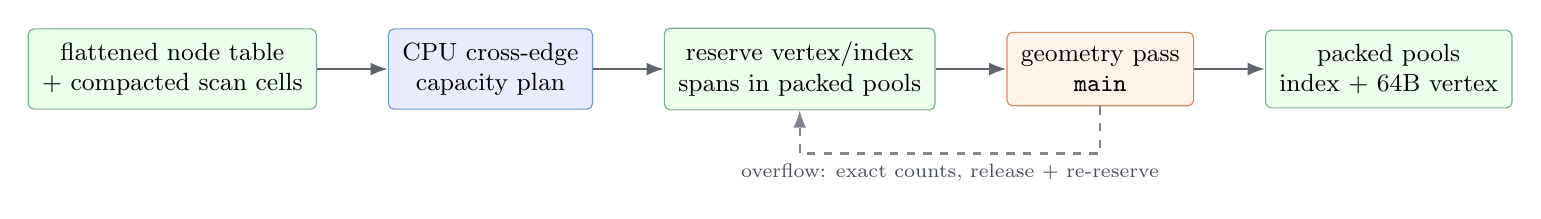
\begin{tikzpicture}[node distance=6mm and 9mm,font=\small]
  \node[io] (in) {flattened node table\\+ compacted scan cells};
  \node[cpu,right=of in] (cap) {CPU cross-edge\\capacity plan};
  \node[io,right=of cap] (host) {reserve vertex/index\\spans in packed pools};
  \node[gpu,right=of host] (pass) {geometry pass\\\code{main}};
  \node[io,right=of pass] (out) {packed pools\\index + 64B vertex};
  \draw[arrow] (in)--(cap);
  \draw[arrow] (cap)--(host);
  \draw[arrow] (host)--(pass);
  \draw[arrow] (pass)--(out);
  \draw[darrow] (pass.south) -- ++(0,-6mm) -| node[pos=0.25,below,note]{overflow: exact counts, release + re-reserve} (host.south);
\end{tikzpicture}}
\caption{The single geometry dispatch.  The CPU sizes both spans from the
cross-edge topology before submission; the shader appends indices directly
and writes each referenced vertex payload once.  A defensive overflow is
reported through counters and resolved by growing only this chunk's span.}
\label{fig:geometrypass}
\end{figure}

\subsection{Overflow without out-of-bounds writes}

The shader still reserves an index base with \code{atomicAdd} and writes the
triangle only when
\begin{equation}
  \text{base}+3 \le I_{\text{cap}}
  \quad\land\quad
  \text{extent} \le V_{\text{cap}}.
\end{equation}
On failure it increments an overflow counter and drops the triangle, but it
has already advanced the index counter by three and updated the maximum
referenced slot.  The host therefore reads back the exact index requirement
and vertex extent without any write outside the reserved span.  It releases
that chunk's span and asks the provider for the grown capacities; the retry
is limited to this chunk and normally the first grown attempt succeeds.  A
fixed-array overflow or a corner without a host-assigned slot is not
retryable: that indicates a flattening disagreement, so the chunk is
failed.

\subsection{Determinism}

The walker uses atomics for the index append, the overflow counters, and
the per-node vertex election.  Triangle order at the end of the index
stream is therefore non-deterministic when two scan cells emit
concurrently.  Does that matter?  The rendered triangle \emph{set} is
deterministic, and each corner carries its host-assigned slot.  The
renderer does not care about triangle order.  The vertex slots are assigned
by the host in node-table order, not by emission order, so a rebuild
produces the same vertex buffer for the same node table.  Ray tracing and
shadow maps are order-independent.  The only observable order is the
index stream, which is internal to the chunk.

\subsection{Precision strategy}

The shader is a direct translation of the CPU arithmetic:
\begin{itemize}
\item corner order, edge order, and QEF accumulation order are identical;
\item the trilinear lerp uses the same guarded branch;
\item the QEF uses the same Cramer solve and the same $10^{-2}$ regularizer;
\item the gradient and QEF use \code{precise} to prevent FMA contraction;
\item the sample nudge uses \code{nextafter} semantics, including the
  subnormal guard at zero.
\end{itemize}
The goal is not merely a visually similar mesh; it is a mesh that the
offline exporter can compare triangle-by-triangle.  Where the GPU cannot
guarantee the same order (atomic append), the triangle set is still
identical because the walker's per-cell output is independent.

\section{Flattening the octree neighbourhood}
\label{sec:flatten}

\subsection{What the shader needs}

A chunk's scan cell can query a neighbouring cell at a coarser or finer
LoD, possibly in a neighbouring chunk.  The shader cannot walk pointers, so
the host must provide a node table that contains every cell the walk can
reach.  The table must include:

\begin{enumerate}
\item the world root at index 0 (the shader's descent anchor);
\item the root-to-chunk ancestor path, with root-consistent cubes;
\item all descendants of the chunk down to the target LoD;
\item all coarser nodes in the one-cell margin around the chunk, plus
  their children, because an edge sample can cross the boundary and land
  in a coarser neighbour;
\item a child index per node (or $-1$ when absent);
\item one dense vertex slot per surface node in the table.
\end{enumerate}

\begin{figure}[htbp]
\centering
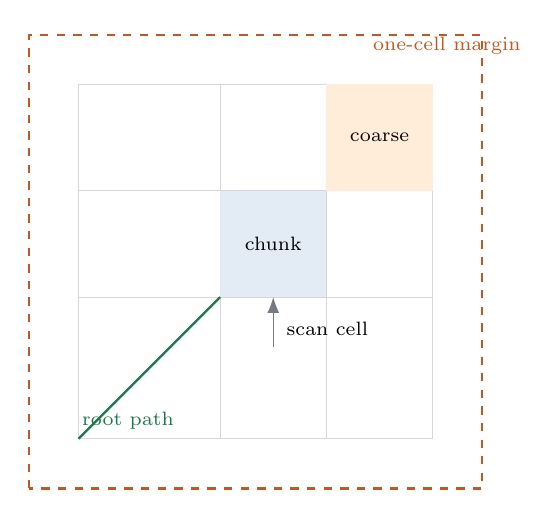
\begin{tikzpicture}[scale=0.9]
  % chunk grid
  \draw[grid] (0,0) rectangle (5,5);
  \draw[grid] (2,0)--(2,5); \draw[grid] (3.5,0)--(3.5,5);
  \draw[grid] (0,2)--(5,2); \draw[grid] (0,3.5)--(5,3.5);
  \fill[accent!12] (2,2) rectangle (3.5,3.5);
  \node[font=\scriptsize] at (2.75,2.75) {chunk};
  % margin
  \draw[accent2,thick,dashed] (-0.7,-0.7) rectangle (5.7,5.7);
  \node[font=\scriptsize,accent2] at (5.2,5.55) {one-cell margin};
  % root path
  \draw[good,thick] (0,0)--(0.8,0.8)--(2,2);
  \node[font=\scriptsize,good] at (0.7,0.25) {root path};
  % neighbor coarse
  \fill[orange!15] (3.5,3.5) rectangle (5,5);
  \node[font=\scriptsize] at (4.25,4.25) {coarse};
  % arrows
  \draw[-{Latex[length=2mm]},ink!60] (2.75,1.3) -- (2.75,2.0);
  \node[right,font=\scriptsize] at (2.8,1.55) {scan cell};
\end{tikzpicture}
\caption{The flattened neighbourhood.  The chunk subtree is walked to the
target rung; the one-cell margin is included so edge samples that cross
the boundary can resolve coarser neighbours.  Index 0 is always the world
root, because the shader's descent starts there for samples outside the
chunk anchor cube.}
\label{fig:flatten}
\end{figure}

\subsection{Root-consistent ancestor chain}

The host replays the child index from the world root to the chunk:
\begin{lstlisting}[caption={Ancestor chain replay.},label={lst:chain}]
cube = rootCube; node = root;
chain.push({node, cube});
while (node != chunk) {
    i = cube.getChildIndex(chunkCenter);
    node = children[i];
    cube = cube.getChild(i);
    chain.push({node, cube});
}
\end{lstlisting}
The replay is necessary because a cached chunk cube may have accumulated
float drift.  The shader will compute its own child indices from the world
root, so the host must use exactly the same arithmetic.  If the chain
cannot be replayed (stale node, missing child), the chunk is marked
\code{Unavailable}; there is no CPU fallback.

\subsection{Descending the table}

The table is built from the chain root.  For each node, the host writes:
\begin{center}
\begin{tabular}{@{}ll@{}}
\toprule
Buffer & Contents\\
\midrule
\code{sdf0, sdf1} & two \code{vec4}s of corner samples\\
\code{cubeMinSize} & \code{vec4(cubeMin, cubeSize)}\\
\code{meta} & \code{ivec4(lod, type, brush, flags)}\\
\code{hsv} & \code{vec4(hsv, textureType)}, \code{vec4(data,0,0)}\\
\code{child03, child47} & two \code{ivec4}s of child indices\\
\code{cells} & compacted scan-cell node ids\\
\bottomrule
\end{tabular}
\end{center}
The layout is 128 bytes per node: $4\times4$ floats for SDFs, $4$ floats
for the cube, $4$ ints for metadata, $8$ floats for HSV/mapping, and $8$
ints for children.  It is uploaded into host-visible coherent buffers; the
shader reads it through storage-buffer descriptors.

\subsection{The scan-cell list}

The scan list contains cells exactly at the target rung that have at least
one crossing edge.  The host counts the crossing edges per cell while it
builds the list:
\begin{equation}
  \text{crossEdges}(c) =
  \#\{(i,j)\in\text{SDF\_EDGES} :
      \operatorname{sign}(d_i)\ne\operatorname{sign}(d_j)\},
\end{equation}
with $+\infty$ counting as non-negative.  This is not the same as
\code{type == Surface}: a negative-plus-infinity cell is typed Solid yet
can emit an edge.  Filtering by type would silently drop those edges.

The same pass produces the index-capacity hint used by the geometry
dispatch:
\begin{equation}
  I_{\text{hint}} =
  6 \sum_{c\in\text{cells}}
      \operatorname{clamp}\!\left(
        \frac{\text{cellSize}(c)}{m},1,64\right)
      \cdot\text{crossEdges}(c),
\end{equation}
where $m$ is the smallest cube in the flattened table.  A segment expands
to at most two triangles of three indices; the clamp is the shader's break
list capacity.  This is a topology bound, not a statistical estimate.  If
it is nevertheless exceeded, the shader reports the exact requirement and
the host grows only that chunk's span.

\subsection{The descent anchor}

The shader's \code{findCellAt} descends from the root.  A per-sample root
descent would be expensive, so the host supplies \code{fromId}: the first
node on the chunk path whose stored LoD is at most the target LoD.  For any
sample inside that node's cube, starting the descent there is
bit-identical to starting at the root, because no ancestor of the anchor
is a stop node.  Samples in the margin outside the anchor fall back to the
root.  This is a pure optimization; the result is the same.

\subsection{Why the margin is one cell}

An edge sample point is a corner of a scan cell, nudged outward by one ulp
in two axes.  The neighbouring quadrant cell can be one cell larger than
the scan cell (a coarse ancestor).  The flattening domain is therefore
\begin{equation}
  [\mathbf{c}_{\min}-\ell,\; \mathbf{c}_{\max}+\ell],
\end{equation}
where $\ell$ is the largest target-rung cell size in the subtree,
\emph{including non-surface cells that were compacted out of the scan
list}.  Deriving the margin from the compacted list would under-estimate
the largest neighbour and could omit a cell the walk samples.

\subsection{Vertex slots}

Every node whose \code{type} is \code{Surface} receives a dense slot in
table order:
\begin{equation}
  \text{flags} \mathrel{|}= (s+1)\ll1.
\end{equation}
Bit 0 remains the leaf flag.  The shader decodes
\begin{equation}
  s = (\text{flags}\gg1)-1.
\end{equation}
The count is the dense slot address space, an exact upper bound on every
index the shader can write.  It is not the number of vertices actually
produced: the geometry pass writes the payload only for slots referenced by
a triangle, and the published span is trimmed to the highest referenced
slot plus one.  Unreferenced slots between zero and that extent remain holes
in the reserved span, so the per-chunk profile reports both the written
vertex count and the published extent.

\subsection{Table order and determinism}

The table order is fixed by the traversal: root, chunk subtree in
child-index order, then the margin descent.  The slot assignment follows
that order.  A rebuild with the same tree produces the same slots.  The
renderer relies on this for the packed-pool span and for the ray-tracing
BLAS, which references the same base vertex and index ranges.

\subsection{Failure modes}

Flattening can fail for only a few reasons:
\begin{itemize}
\item the chunk node is not reachable from the root (stale parameters);
\item the chain is deeper than 200 (a corrupt tree);
\item the chunk has no crossing scan cell, or no surface node in the
  flattened table owns a slot (a valid empty chunk, not a failure);
\item the table is missing a child block the descent needs.
\end{itemize}
The first, second, and fourth mark the chunk \code{Unavailable}; the
caller skips it and logs.  The third returns a valid empty input, the
geometry pass is not dispatched, and the publisher settles the empty
revision.

\section{Stage 0: the GPU walk}
\label{sec:gpuwalk}

\subsection{Invocation model}

The walk dispatch has one invocation per compacted scan cell:
\begin{equation}
  \text{groups} = \left\lceil \frac{|\text{cells}|}{64} \right\rceil,
\end{equation}
with a local size of 64.  The shader starts from
\code{gl_GlobalInvocationID.x}; if it is beyond the cell count, it
returns.  All per-invocation state is private:
\begin{itemize}
\item break list (64 floats),
\item local break list (32 floats),
\item task stack (256 intervals),
\item QEF position memo (8 entries),
\item overflow flag and diagnostic counters.
\end{itemize}
No workgroup shared memory is needed.  This makes the pass portable across
devices with small shared-memory budgets and avoids workgroup
synchronization.

\subsection{Node accessors}

The shader wraps the eight storage buffers in typed accessors:
\begin{lstlisting}[style=glsl,caption={Node accessors (abridged).},label={lst:accessors}]
float nodeSdf(uint id, int i) { return (i < 4) ? sdf0[id][i] : sdf1[id][i-4]; }
int nodeType(uint id)   { return meta[id].y; }
int nodeBrush(uint id)  { return meta[id].z; }
int nodeSlot(uint id)   { return int(meta[id].w >> 1) - 1; }
vec3 nodeMin(uint id)   { return cubeMinSize[id].xyz; }
float nodeSize(uint id) { return cubeMinSize[id].w; }
int nodeChild(uint id, int i) { ... }
\end{lstlisting}
The table is a flat array; there are no pointers.  The accessors are
inlined by the compiler.

\subsection{\code{findCellAt}}

The descent mirrors the CPU walker:
\begin{lstlisting}[style=glsl,caption={The root-to-cell descent.},label={lst:findcell}]
Cell findCellAt(vec3 pos) {
    if (!worldContains(pos)) return INVALID;
    uint idx = pc.fromId >= 0 ? pc.fromId : 0;
    if (pos outside anchor cube) idx = 0;
    while (!nodeIsLeaf(idx) && nodeLod(idx) > pc.targetLod) {
        ivec3 half = nodeMin(idx) + 0.5*nodeSize(idx);
        int child = (pos.x >= half.x ? 4 : 0)
                  + (pos.y >= half.y ? 2 : 0)
                  + (pos.z >= half.z ? 1 : 0);
        int c = nodeChild(idx, child);
        if (c < 0) return INVALID;
        idx = c;
    }
    return Cell(idx, nodeMin(idx), nodeSize(idx));
}
\end{lstlisting}
The stop condition is ``leaf or stored LoD at most target''.  The stored
LoD is +1 shifted, exactly as on the CPU.  Starting at \code{fromId} is
valid only for positions strictly inside the anchor cube; a point on the
upper face must follow the sibling branch, so the test uses a strict upper
bound.

\subsection{Edge span construction}

For each of the twelve cube edges, the shader loads the two corner signs.
If they are equal, the edge is inactive.  Otherwise it builds an
\code{EdgeSpan}.  The varying axis is the component with the largest
absolute corner difference (exact for an axis-aligned cube).  The two other
axes are the fixed $u,v$ axes.  The span's epsilon is
\begin{equation}
  \epsilon = \max(\text{worldSize}, L)\cdot10^{-6},
\end{equation}
and the boundary sample offset is
\begin{equation}
  \delta = \max(L\cdot10^{-3},10^{-6}).
\end{equation}
The epsilon is used for duplicate rejection and sign-change tests; the
offset is used when a sample sits exactly on a cell face.

\subsection{The ulp nudge and the zero guard}

Sampling a point exactly on a cell face is ambiguous: the two cells both
claim it.  The shader nudges the fixed coordinates by one float in the
direction of the quadrant.  At zero, \code{nextafter(0,+inf)} is a
subnormal; FTZ GPUs flush it to zero, and the negative quadrant then
resolves into the positive cell.  The shader detects a subnormal nudge and
uses a small normal offset instead.  This is a small detail with a large
visual consequence: without it, the surface disappears along the world
$x=0$, $y=0$, and $z=0$ planes.

\subsection{The scan loop}

For each active edge the walk:
\begin{enumerate}
\item initializes the global break list with the span endpoints;
\item calls \code{collectBreaks};
\item sorts and uniques the global list;
\item iterates consecutive breaks and calls \code{emitSegment} for each
  interval wider than $2\epsilon$.
\end{enumerate}
This is exactly the CPU loop.  The only difference is that the CPU stores
the breaks in a \code{std::vector} and the GPU uses fixed arrays.

\subsection{Diagnostics}

Two counters are accumulated only when \code{VULKAN_SETUP_DIAG} is set:
\code{findCellCalls} and \code{reuseHits}.  They are summed locally and
published with one atomic pair per scan cell, so the diagnostic path does
not add a per-call atomic.  The normal path has a predictable branch and no
counter traffic.

\begin{figure}[htbp]
\centering
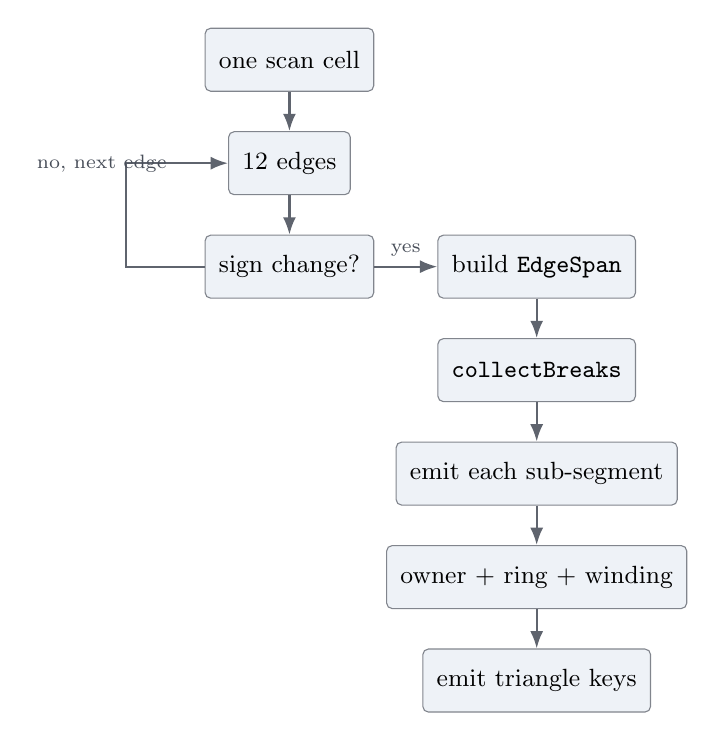
\begin{tikzpicture}[node distance=5mm and 8mm,font=\small]
  \node[box] (cell) {one scan cell};
  \node[box,below=of cell] (edges) {12 edges};
  \node[box,below=of edges] (active) {sign change?};
  \node[box,right=of active] (span) {build \code{EdgeSpan}};
  \node[box,below=of span] (breaks) {\code{collectBreaks}};
  \node[box,below=of breaks] (segments) {emit each sub-segment};
  \node[box,below=of segments] (poly) {owner + ring + winding};
  \node[box,below=of poly] (tri) {emit triangle keys};
  \draw[arrow] (cell)--(edges); \draw[arrow] (edges)--(active);
  \draw[arrow] (active)--node[above,note]{yes}(span);
  \draw[arrow] (span)--(breaks); \draw[arrow] (breaks)--(segments);
  \draw[arrow] (segments)--(poly); \draw[arrow] (poly)--(tri);
  \draw[arrow] (active.west) -- ++(-1.0,0) |- node[pos=0.75,left,note]{no, next edge} (edges.west);
\end{tikzpicture}
\caption{One scan-cell invocation.  Inactive edges are skipped; active
edges are stitched and emitted.  The entire control flow is private to the
invocation.}
\label{fig:scanflow}
\end{figure}

\section{Step-by-step adaptive stitching}
\label{sec:stitch}

\subsection{The exact problem}

Consider an active edge shared by four cells.  In a non-adaptive mesh, the
four cells all have the same size and the edge contributes one segment.  In
an adaptive mesh, the four cells can be a mix of coarse and fine cells.
The edge can cross a boundary between two cells at any coordinate.  The
correct mesh splits the edge at every such boundary and emits one segment
per sub-interval.  The two chunks on either side of a chunk boundary must
produce the same split list; otherwise their rings disagree and a crack
opens.

\subsection{Why a fixed stitching table is not used}

A transvoxel-style table enumerates the finite set of cell configurations
and gives a triangulation for each.  That works when the LoD difference
across a boundary is at most one level and the cell sizes are known.  Here
the difference can be arbitrary (a coarse root cell next to a fine leaf),
the tree is sparse, and the cell sizes are continuous.  A table would have
to enumerate a combinatorial set of nested cells.  The break collector
instead computes the split from the actual cell boundaries, which is
configuration-independent.

\subsection{The recursion, formally}

Let $E$ be an edge span and $[a,b]\subseteq E$ an interval.  Define
\begin{equation}
  B(a,b) = \{\, c_x \mid \text{quadrant cell } c \text{ at } (a+b)/2
  \text{ contributes } c_{\min,x} \text{ or } c_{\max,x} \,\}
\end{equation}
restricted to values strictly inside $(a,b)$ and not within $\epsilon$ of
an existing break.  Then:
\begin{enumerate}
\item append every interior value of $B(a,b)$ to the global break list;
\item for each consecutive pair $a=t_0<t_1<\cdots<t_k=b$, recurse on
  $[t_{i-1},t_i]$ if it is longer than $2\epsilon$.
\end{enumerate}
The recursion terminates because each level inserts at least one break, or
the interval is shorter than $2\epsilon$.  In practice it terminates after
one or two levels: the cell boundaries are powers of two and the interval
is the current edge segment.

\subsection{The GPU stack}

The CPU implementation uses recursion.  The shader replaces it with a LIFO
stack of intervals.  The CPU's exact order is:
\begin{itemize}
\item append all interior breaks first;
\item then recurse into the sub-intervals from left to right.
\end{itemize}
The shader reproduces this by pushing sub-intervals in reverse order:
\begin{lstlisting}[style=glsl,caption={Reverse push preserves the CPU order.},label={lst:push}]
for (int i = localCount - 1; i >= 1; --i)
    pushTask(local[i-1], local[i]);
\end{lstlisting}
Because the stack pops the last pushed interval first, it visits
$[t_0,t_1]$ before $[t_1,t_2]$, and fully expands each before the next.
The global break list is identical to the CPU's.

\subsection{The sample offset}

The quadrant samples are nudged by $\delta$ in the two fixed axes.  The
nudge is not a random jitter: it is a deterministic one-ulp move toward the
quadrant.  The two axes are chosen by \code{edgeAxes}: for an $x$-edge the
fixed axes are $y,z$; for a $y$-edge they are $x,z$; for a $z$-edge they
are $x,y$.  The four quadrant signs are fixed by the \code{quadrantSigns}
table:
\begin{center}
\begin{tabular}{@{}c|cccc@{}}
\toprule
axis & $q_0$ & $q_1$ & $q_2$ & $q_3$\\
\midrule
$x$ & $(-1,-1)$ & $(-1,+1)$ & $(+1,+1)$ & $(+1,-1)$\\
$y$ & $(-1,-1)$ & $(+1,-1)$ & $(+1,+1)$ & $(-1,+1)$\\
$z$ & $(-1,-1)$ & $(-1,+1)$ & $(+1,+1)$ & $(+1,-1)$\\
\bottomrule
\end{tabular}
\end{center}
The actual table is flattened as
\code{QS[axis*8 + quadrant*2 + {0,1}]}; its values are shown above.

\subsection{Break capacities and overflow}

The fixed capacities are a hard contract.  A scan cell with more than 64
breakpoints, or an interval with more than 32 local breaks, or a recursion
stack deeper than 256 intervals is not expected for the engine's cell
sizes, but it is still possible for a pathological SDF.  The shader does
not truncate:
\begin{itemize}
\item \code{noteOverflow()} sets \code{gOverflow};
\item the cell stops emitting;
\item \code{overflowCount} is incremented;
\item the host sees the counter and fails the chunk.
\end{itemize}
The host retries the chunk after the tree edit or reports it as skipped.
It never publishes a partial index stream.  This is an important
difference from a ``best effort'' GPU mesher: a silent truncation would be
a hole in the terrain that is hard to diagnose.

\subsection{The global break list}

The global list is sorted and deduplicated by insertion sort and a linear
unique pass.  The lists are small (at most 64 entries), so an $\Oh(n^2)$
sort is faster than a library sort and, more importantly, has a
deterministic order.  Equality uses the edge epsilon:
\begin{equation}
  |b_i-b_j|\le \epsilon \quad\Rightarrow\quad \text{duplicate}.
\end{equation}
The sort is stable for equal keys because the insertion sort only moves
strictly greater values.  This matches the CPU's \code{std::sort} behaviour
for these list sizes and keeps the emitted triangle order deterministic.

\subsection{Owner and quadrant sampling}

For each sub-segment the shader samples the four quadrants at its
midpoint.  It does not reuse the quadrant cells from the break collection:
the midpoint of a sub-segment is a different position and may fall in a
different cell.  The owner is selected by the ordering rule of
\Cref{sec:cpuwalk}.  The owner's interpolated field at the segment
endpoints decides the winding.  If the owner's interpolation degenerates
(both endpoints get the same sign because a zero lies exactly on a corner),
the producing cell's endpoint signs are used instead.  Those signs are
authoritative because the producing cell only scans edges with a sign
change.

\subsection{Consequences}

The stitching step is what makes it legal to publish every LoD rung and let
the renderer choose one per region.  Without it, the mesh would be
crack-free only within a single rung; at rung transitions the surface would
have T-junctions and visible seams.  With it, the coarse and fine sides of
a boundary agree on the edge split and on the owner, so their duplicated
boundary quads have identical vertex order and identical triplanar plane.
This is also why the chunk-border guard in the simplifier is necessary:
the stitching can resolve interior LoD changes, but it cannot resolve a
difference in the chunk's own boundary cells because the two chunks never
share a node table.

\section{Polygon reconstruction, winding, and triangle emission}
\label{sec:polygon}

\subsection{From four quadrants to a ring}

For a sub-segment the shader resolves four quadrant cells.  Not all of
them are surface cells: a coarse cell can have no zero crossing at the
sample.  The algorithm:
\begin{enumerate}
\item iterate quadrants in the fixed order $q_0,\ldots,q_3$;
\item skip non-surface cells;
\item compute the cell's dual vertex position with the memoized QEF;
\item reject a cell if its node id or position duplicates an already
  collected cell (within the edge epsilon);
\item stop at four collected cells.
\end{enumerate}
The deduplication is not merely an optimization.  A coarse ancestor can
appear in two opposite quadrants of the ring, especially on world-axis
cell boundaries where the sample nudge stays inside the same large cell.
The old code removed only adjacent duplicates and then aborted the whole
segment if any duplicate remained; that is exactly why triangles were
missing along the $x=0$, $y=0$, and $z=0$ planes.  Deduplicating against
all collected cells keeps the remaining 3 or 4 corners and preserves their
order.

\subsection{Rotating the owner to the front}

The ring is rotated so the owner cell is first:
\begin{lstlisting}[style=glsl,caption={Owner rotation.},label={lst:rotate}]
find k with ring[k].id == owner.id or ring[k].pos == owner.pos;
if (k > 0) rotate ring left by k;
\end{lstlisting}
Both chunks on either side of a boundary resolve the same owner (the
ordering key is global), so their duplicated boundary quads get the same
rotation.  Without this, the same quad would be triangulated from different
anchors on the two sides, producing different triplanar planes and
z-fighting along the seam.

\subsection{Three-ring and four-ring fans}

A three-ring emits one triangle:
\begin{equation}
  (r_0,r_1,r_2).
\end{equation}
A four-ring emits two:
\begin{equation}
  (r_0,r_1,r_2), \quad (r_0,r_2,r_3).
\end{equation}
If the owner's start sign is positive (outside), the order is reversed:
\begin{equation}
  (r_0,r_2,r_1), \quad (r_0,r_3,r_2).
\end{equation}
This is a fan around the owner.  A ring with fewer than three cells emits
nothing; it is a boundary case where the surface only touches one or two
quadrants.

\subsection{The winding oracle}

The winding is not derived from the triangle normal.  It is derived from
the SDF sign at the segment start, evaluated with the owner's trilinear
field:
\begin{equation}
  \text{solidAtStart} = \bigl(d_{\text{owner}}(a) < 0\bigr).
\end{equation}
If the owner's interpolation returns $+\infty$, the producing cell's
endpoint sign is used.  The producing cell is the cell that scanned the
edge, and it only scans edges whose own corner signs differ; those signs
are therefore authoritative for existence.

Why not use the QEF normal?  At coarse LoD a cell can have only one or two
crossing edges, and the QEF normal is poorly constrained.  A triangle
wound from a noisy normal can flip at a LoD boundary, making the surface
black or invisible from one side.  The sign oracle is independent of the
normal and robust across cell sizes.

\subsection{Degenerate triangles}

Before appending, the shader compares the three dual positions:
\begin{equation}
  \|p_i-p_j\| \le \epsilon \quad\Rightarrow\quad \text{drop}.
\end{equation}
This catches two cases:
\begin{itemize}
\item two cells collapsed to the same QEF position (a thin sliver);
\item a cell with an exact-zero corner snapped to the corner, coinciding
  with a neighbouring cell's vertex.
\end{itemize}
A zero-area triangle would break normals, shadow-map rasterization, and
ray-triangle intersections.  Dropping it is safer than emitting it.

\subsection{Direct index append and lazy vertices}

The triangle is appended straight into the chunk's index span:
\begin{lstlisting}[style=glsl,caption={Index append.},label={lst:indexappend}]
uint base = atomicAdd(indexCount, 3u);
int s0 = nodeSlot(c0.id), s1 = nodeSlot(c1.id), s2 = nodeSlot(c2.id);
if (s0 < 0 || s1 < 0 || s2 < 0) { atomicAdd(invalidSlotCount, 1u); return; }
uint extent = max(max(s0, s1), s2) + 1u;
atomicMax(vertexExtent, extent);
if (base + 3u > pc.indexCapacity || extent > pc.vertexCapacity) {
    atomicAdd(indexOverflow, (base + 3u > pc.indexCapacity) ? 1u : 0u);
    atomicAdd(vertexOverflow, (extent > pc.vertexCapacity) ? 1u : 0u);
    atomicAdd(droppedCount, 1u);
    return;
}
poolIdx[pc.indexBase + base + 0u] = uint(s0);
poolIdx[pc.indexBase + base + 1u] = uint(s1);
poolIdx[pc.indexBase + base + 2u] = uint(s2);
writeVertexOnce(c0.id, s0);
writeVertexOnce(c1.id, s1);
writeVertexOnce(c2.id, s2);
\end{lstlisting}
The atomic only reserves the base; the three index writes are private.
The counter advances by three even when the triangle does not fit, so the
host reads the exact index requirement for the overflow-growth retry.  No
write below the capacity check is ever outside the reserved span, so an
overflow cannot corrupt another chunk.

The vertex payload is a pure function of its node.  Many corners reference
the same surface node, so the shader elects one writer per node with an
\code{atomicExchange} on the device-local \code{nodeWritten} buffer, which
is cleared before every dispatch.  The elected invocation writes the
64-byte payload and increments \code{vertexWriteCount}; the others skip it.
By the time the dispatch completes, every referenced payload is therefore
written exactly once.

\subsection{Triangle order and visual invariance}

The order of triangles in the index stream is the order in which scan cells
happen to append.  Different GPUs, workgroup schedules, or occupancy can
produce a different order.  This is acceptable because:
\begin{itemize}
\item the triangle set is identical (each cell's output is independent);
\item the renderer draws the whole index range, not a prefix;
\item the shadow map, depth prepass, and ray tracing are order-independent;
\item the vegetation and fire anchors are keyed by chunk/node, not by
  triangle index.
\end{itemize}
The only place order matters is debugging: a diff of two index streams
must be order-insensitive.  The engine's self-check compares triangle sets,
not raw arrays.

\subsection{The boundary quad}

A duplicated boundary quad is emitted by both neighbouring chunks.  Both
copies must be identical in position, order, and material.  The engine
guarantees this by:
\begin{enumerate}
\item using the same owner ordering key (size, min, node index);
\item sampling the same four quadrants (the neighbour's node table contains
  the same cells);
\item using the same QEF arithmetic and the same edge epsilon;
\item rotating the owner to the front.
\end{enumerate}
The duplicate triangles are not removed at the chunk level; the renderer
draws both.  They coincide exactly, so the depth test resolves the
z-fight.  Removing them would require a cross-chunk dedup pass and would
reintroduce a seam if the dedup key differed.

\section{Step-by-step QEF vertex solve and payload}
\label{sec:qef}

\subsection{Why a QEF instead of an average}

A Surface Nets vertex is often placed at the average of the edge
crossings.  That is cheap but smooths sharp features: a box corner becomes
a rounded blob.  A QEF fits a point to the tangent planes of the crossings,
which preserves sharp edges better while still producing one vertex per
cell.  The engine regularizes the QEF toward the mass point so an
underconstrained cell does not explode.

\subsection{The twelve crossings}

For each edge $(i,j)$ with finite endpoints and opposite signs:
\begin{equation}
  t = \clip\left(\frac{d_i}{d_i-d_j},0,1\right),
  \quad
  \mathbf{p} = (1-t)\mathbf{p}_i + t\mathbf{p}_j,
  \quad
  \mathbf{n} = \operatorname{normalize}\bigl((1-t)\mathbf{n}_i+t\mathbf{n}_j\bigr).
\end{equation}
The corner normals $\mathbf{n}_i$ are the analytic gradients of the
trilinear field at the corner.  The edge normal is the interpolation of
the two corner normals, not the normalized edge direction.  This is what
makes the QEF preserve the smooth surface normal.

\subsection{Accumulation}

The normal equations are accumulated:
\begin{align}
  A &= \sum_e \mathbf{n}_e\mathbf{n}_e^{T} + \epsilon I,\\
  \mathbf{b} &= \sum_e \mathbf{n}_e(\mathbf{n}_e\cdot\mathbf{p}_e)
             + \epsilon\bar{\mathbf{p}}.
\end{align}
where $\bar{\mathbf{p}}$ is the average crossing and $\epsilon=10^{-2}$.
The matrix is symmetric positive semidefinite; the shift makes it
invertible.  Cramer's rule is used because it is branch-free and matches
the CPU's GLM evaluation order.  A determinant below $10^{-6}$ returns zero
and the caller falls back to the mass point.

\subsection{Corner snap}

If any corner SDF is exactly zero, the vertex is snapped to that corner:
\begin{equation}
  \mathbf{x} = C_i.
\end{equation}
Why?  Neighbouring cells sharing the corner would otherwise solve slightly
different QEF systems (their normals and crossings differ in the low bits)
and their vertices would drift apart, splitting the shared edge into two
one-sided edges.  Snapping to the exact corner makes every incident cell
produce the same bits.  This is a classic dual-contouring robustness fix
and it is essential for watertight terrain.

\subsection{Sentinel handling}

An edge with an infinite endpoint is skipped.  If no usable edge remains
but there are finite sign-changing edges blocked by a sentinel, the shader
averages the finite crossings instead of returning the cell centre.  The
fallback keeps the vertex on the real surface segment rather than floating
in the middle of the cell.

\subsection{Clamping}

The result is clamped to the cell:
\begin{equation}
  \mathbf{x} = \clip(\mathbf{x}, \mathbf{c}, \mathbf{c}+L).
\end{equation}
A QEF solution outside the cell would make the dual mesh non-manifold and
could place a vertex inside a neighbouring solid.  The clamp is the last
line of defence after regularization.

\subsection{Memoization}

The shader memoizes up to eight QEF positions per invocation.  A single
edge segment queries the same cells several times (owner selection, dedup,
rotation, fan).  The memo is a linear scan over eight entries; it is
value-identical to recomputing because the QEF is a pure function of the
node's eight corners and cube.  If the memo is full, the slot is chosen by
\code{id mod 8}; a collision simply evicts an older entry.

\subsection{The payload}

Stage 1 writes the final vertex from the node id:
\begin{lstlisting}[style=glsl,caption={Vertex payload layout.},label={lst:payload}]
uint o = (pc.vertexBase + slot) * 4u;
poolVerts[o+0] = vec4(p, 1.0);
poolVerts[o+1] = vec4(1.0, 1.0, data);
poolVerts[o+2] = vec4(n, uintBitsToFloat(uint(brush)));
poolVerts[o+3] = vec4(uintBitsToFloat(uint(type)), h);
\end{lstlisting}
The vertex is 64 bytes:
\begin{center}
\begin{tabular}{@{}c|l@{}}
\toprule
Word & Bytes\\
\midrule
0 & position.xyz (12) + color.x (4)\\
1 & color.yz (8) + texCoord.xy (8)\\
2 & normal.xyz (12) + brushIndex bits (4)\\
3 & textureType bits (4) + hsv (12)\\
\bottomrule
\end{tabular}
\end{center}
The \code{textureType} is stored as integer bits, not as a float value.
The vertex input attribute is \code{R32\_SINT}, and the ray-tracing path
uses \code{floatBitsToInt}; writing a numeric float would decode to a
garbage mapping mode and drop every non-triplanar vertex.

\subsection{One vertex per node}

Every surface node in the flattened table gets a vertex, including nodes
that the index stream never references.  This is intentional:
\begin{itemize}
\item it makes slot assignment a simple table order;
\item it makes the span size known from the host count;
\item it lets the finalize pass write one vertex per invocation without a
  compaction pass.
\end{itemize}
The wasted bytes are bounded by the number of surface nodes in the
neighbourhood and are small compared with the triangle stream.

\section{Stage 1: finalize the index and vertex streams}
\label{sec:finalize}

\subsection{One dispatch, two tails}

After the host reserves the spans, the finalize dispatch runs with
\begin{equation}
  \text{work} = \text{indexCount} + \text{nodeCount}.
\end{equation}
The first \code{indexCount} invocations write the index stream; the
remaining \code{nodeCount} invocations write the vertex payload:
\begin{lstlisting}[style=glsl,caption={Finalize stage.},label={lst:finalize}]
void finalizeStage() {
    uint gi = gl_GlobalInvocationID.x;
    if (gi < pc.indexCount) { writeIndex(gi); return; }
    uint node = gi - pc.indexCount;
    if (node >= pc.nodeCount) return;
    writeVertexForNode(node);
}
\end{lstlisting}
The index range is first because it is usually much larger than the node
count.  The two ranges are disjoint, so one dispatch covers both without a
barrier between them.

\subsection{Index remap}

For index $i$, the raw key is the node id:
\begin{equation}
  \text{slot} = \text{nodeSlot}(\text{rawKeys}[i]).
\end{equation}
If the slot is negative, the host's slot assignment and the walk disagree.
The shader increments \code{droppedCount} and fails the chunk rather than
writing slot 0.  Writing 0 would silently connect the corner to an
arbitrary vertex and produce a stretched triangle.

\subsection{Vertex reconstruction}

The vertex is rebuilt from the node, not from the walk's temporary cell:
\begin{enumerate}
\item QEF position from the node's eight corners and cube;
\item analytic normal at that position;
\item brush, falling back to the chunk's \code{fromBrush} when the node's
   brush is the discard sentinel;
\item HSV tint, texture type, and mapping data.
\end{enumerate}
This is why the raw key is enough.  The CPU walker keeps the cell payload
in the triangle, but that payload is a pure function of the node.  The GPU
recomputes it in stage 1, which also means the finalize stage does not need
to read the walk's scratch arrays.

\subsection{The index base and alignment}

The chunk's index span is bound with an offset.  The offset must be aligned
to the device's minimum storage-buffer offset alignment.  Since the element size is four
bytes and the alignment can be 256, the host aligns the descriptor offset
down and passes \code{relIndexBase} = the number of index elements between
the aligned offset and the first span element.  The shader writes
\begin{equation}
  \text{poolIdx}[\text{relIndexBase} + i] = \text{slot}.
\end{equation}
The descriptor range is
\begin{equation}
  (\text{relIndexBase} + \text{indexCapacity})\cdot4
\end{equation}
bytes, which includes the padding.  Without the extra padding, the last
elements of the span fall outside the bound range and are never written,
producing stretched triangles from stale pool data.

\subsection{The vertex base and alignment}

The vertex span is handled the same way with a 64-byte stride.  The offset
is aligned down; \code{relVertexBase} accounts for the 0--3 element
padding.  The shader writes
\begin{equation}
  \text{poolVerts}[(\text{relVertexBase} + s)\cdot4 + k].
\end{equation}
The range is
\begin{equation}
  (\text{relVertexBase} + \text{vertexCapacity})\cdot64.
\end{equation}
Because 64 is a multiple of 4 and the largest required alignment is 256, a
span start can be misaligned by at most three vertices.  The padding logic
is exact and costs at most 192 bytes per chunk.

\subsection{Drop accounting}

Every write that cannot fit increments \code{droppedCount}.  The host reads
the counter after the fence.  The chunk is considered valid only when
\begin{equation}
  \text{droppedCount}=0 \quad\land\quad
  \text{overflowCount}=0 \quad\land\quad
  \text{poolVertexCount}\le\text{vertexCapacity}.
\end{equation}
If any check fails, the reserved span is released and the chunk is skipped.
The next edit retries it.  The app never draws a partially written span.

\subsection{The raw-key buffer}

The raw-key buffer is device-local and sized to the key capacity.  It is
written in stage 0 and read in stage 1.  Its lifetime is one topology
submission (two dispatches separated by a host read).  The buffer is
reused across chunks; the host resets the counters before each walk.  The
key capacity is selected from a per-cell hint:
\begin{equation}
  \text{keys} = \min\bigl(\text{cellCount}\cdot25+64,\;2^{23}\bigr).
\end{equation}
A walk that exceeds the hint retries with twice the capacity, up to the
hard limit.  The measured worst chunk is about 3.8 million raw vertices,
below the 8 million limit.

\section{Host orchestration: one submission per chunk}
\label{sec:orch}

\subsection{The driver}

\code{OctreeTopologyCompute::computeResident} is the only entry point.  It
is called by \code{SceneRenderer::buildChunkResident} on a scene worker
thread.  The method holds a mutex for the whole chunk, so two workers never
share the staging buffers or the descriptor set.  The normal path is one
submission:

\begin{enumerate}
\item the host flattens the neighbourhood and derives the cross-edge
  capacities;
\item the provider reserves a vertex/index span in the packed pools;
\item the host uploads the node tables and records one geometry dispatch;
\item the host waits for the fence and reads the counters;
\item the host publishes the span, or grows it once and retries.
\end{enumerate}

\begin{figure}[htbp]
\centering
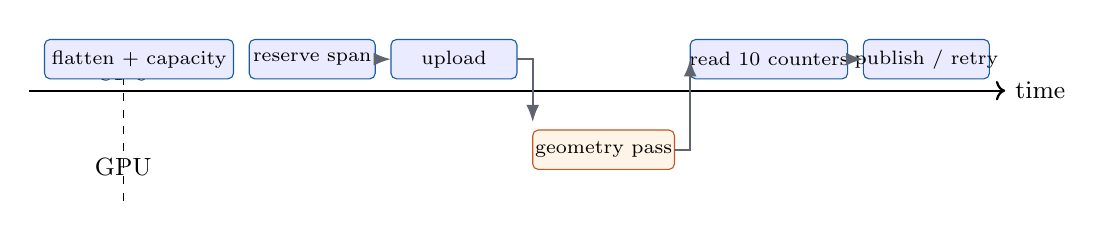
\begin{tikzpicture}[font=\small]
  \draw[->,thick] (0,0) -- (12.4,0) node[right]{time};
  \node[above] at (1.2,0) {CPU};
  \node[above] at (1.2,-1.2) {GPU};
  \draw[dashed] (1.2,-1.4)--(1.2,0.6);
  % CPU work
  \fill[cpu,draw=accent] (0.2,0.15) rectangle (2.6,0.65) node[midway,font=\scriptsize]{flatten + capacity};
  \fill[cpu,draw=accent] (2.8,0.15) rectangle (4.4,0.65) node[midway,font=\scriptsize]{reserve span};
  \fill[cpu,draw=accent] (4.6,0.15) rectangle (6.2,0.65) node[midway,font=\scriptsize]{upload};
  \fill[cpu,draw=accent] (8.4,0.15) rectangle (10.4,0.65) node[midway,font=\scriptsize]{read 10 counters};
  \fill[cpu,draw=accent] (10.6,0.15) rectangle (12.2,0.65) node[midway,font=\scriptsize]{publish / retry};
  % GPU work
  \fill[gpu,draw=accent2] (6.4,-1.0) rectangle (8.2,-0.5) node[midway,font=\scriptsize]{geometry pass};
  % arrows
  \draw[arrow] (4.4,0.4)--(4.6,0.4);
  \draw[arrow] (6.2,0.4)--(6.4,0.4)--(6.4,-0.4);
  \draw[arrow] (8.2,-0.75)--(8.4,-0.75)--(8.4,0.4);
  \draw[arrow] (10.4,0.4)--(10.6,0.4);
\end{tikzpicture}
\caption{One chunk's normal timeline.  The spans are reserved from the CPU
cross-edge bound before submission; the single geometry pass writes the
renderer's pools directly.  The host reads integers after the fence.}
\label{fig:timeline}
\end{figure}

\subsection{The input upload}

The input buffers are host-visible and coherent.  \code{uploadInput} writes:
\begin{itemize}
\item 128 bytes per node for the node table;
\item 4 bytes per cell for the scan list;
\item ten counters (indices, extent, overflow, drops, diagnostics, and the
  distinct vertex write count);
\end{itemize}
and resets the counters.  The upload is not a single \code{memcpy}: the
node record is split across five arrays so the shader can use scalar
layout and avoid a 128-byte struct with alignment surprises.  The
\code{nodeWritten} election buffer is device-local; it is cleared with
\code{vkCmdFillBuffer} immediately before the dispatch, not uploaded from
the host.

\subsection{Capacity management}

The input buffers grow to the largest chunk seen so far:
\begin{equation}
  \text{nodeCap}\ge |\N|,\qquad
  \text{cellCap}\ge |\text{cells}|.
\end{equation}
A grow recreates the buffers and bumps \code{bufferGeneration}.  The
descriptor writer checks the generation and rewrites bindings 0--9 only
when it changes.  In steady state, a chunk with the same capacity reuses
the descriptors and pays zero descriptor writes.  The device-local
\code{nodeWritten} buffer follows \code{nodeCap}; it is not grown per chunk.
The packed vertex/index spans belong to the renderer and are reserved per
chunk.

\subsection{Capacity plan and the provider callback}

The provider is called before the dispatch with a demand derived from the
CPU topology:
\begin{itemize}
\item vertex capacity = \code{activeVertexCount} (dense surface-node slot
  address space);
\item index capacity = $\sum_c 6\cdot\text{segments}(c)\cdot
  \text{crossEdges}(c)$;
\item the cross-edge count and maximum segment span are carried for the
  profile.
\end{itemize}
The provider reserves a stable draw-entry slot and a variable-size span:
\begin{lstlisting}[caption={Span reservation callback (shape).},label={lst:provider}]
GpuMeshSpan span = ir.reserveGpuMeshSpan(chunkId,
    demand.suggestedVertexCapacity, demand.suggestedIndexCapacity,
    &cubeMin, &cubeMax, level, &cubeMin);
target.vertexBuffer = span.vertexBuffer;
target.baseVertex = span.baseVertex;
target.vertexCapacity = span.vertexCapacity;
target.indexBuffer = span.indexBuffer;
target.firstIndex = span.firstIndex;
target.indexCapacity = span.indexCapacity;
target.slotIndex = span.slotIndex;
\end{lstlisting}
If the provider cannot fit the requested capacities, the build fails
without dispatching.  The caller releases the reservation and leaves the
revision uncommitted, so a later opportunity can retry.

\subsection{Overflow growth}

If the shader reports an index or vertex overflow, the service calls the
release callback with the reservation it just failed to use.  The renderer
frees that unpublished span immediately (no draw command references it) and
defers the free of any previously published span through the usual staged
meta flush.  The service then asks the provider for the exact reported
capacities and retries the same chunk with a freshly cleared
\code{nodeWritten} buffer.  At most three attempts are made.  Only this
chunk's spans are released and re-reserved; other chunks and the global
descriptor state are untouched.  A fixed break-list overflow or an invalid
slot fails immediately because capacity cannot fix it.

\subsection{Publication}

After the fence, the host reads the counters.  If the chunk is valid:
\begin{enumerate}
\item \code{publishGpuMeshSpan(slot, vertexExtent, indexCount)} trims the
  reserved span to the referenced extent, frees the tail, and stages the
  draw command + bounds + LoD meta;
\item the scene publisher stores a \code{LoDMesh} with the slot, counts,
  base vertex, first index, bounds, brush, and mapping metadata;
\item the renderer's indirect cull sees the entry on the next frame.
\end{enumerate}
The old span is released only after the new one is published.  The release
is staged for the cull frame after next, so no in-flight cull or draw can
reference a freed range.

\subsection{Why the host reads only counters}

The GPU writes indices and vertices.  The host reads only counters:
\begin{center}
\begin{tabular}{@{}ll@{}}
\toprule
Counter & Use\\
\midrule
\code{indexCount} & indices appended; growth requirement\\
\code{indexOverflow} & triangles rejected by the index span\\
\code{vertexExtent} & published extent; growth requirement\\
\code{vertexOverflow} & triangles rejected by the vertex span\\
\code{vertexWriteCount} & distinct payloads written; utilization\\
\code{invalidSlotCount} & flattening disagreement (fatal)\\
\code{overflowCount} & fixed-capacity recursion failure (fatal)\\
\code{droppedCount} & total rejected triangles\\
\code{findCellCalls} & diagnostics only\\
\code{reuseHits} & diagnostics only\\
\bottomrule
\end{tabular}
\end{center}
No position, normal, or 64-byte vertex ever crosses the bus.  This is the
single most important property of the design: the host cannot accidentally
stall on a vertex readback because there is no vertex readback API.

\subsection{Error policy}

A chunk build can fail in the following ways:
\begin{enumerate}
\item \textbf{flattening unavailable}: the chunk is skipped with a log;
\item \textbf{fixed-array overflow or invalid slot}: the chunk is failed and
  retried after the next edit; it is not partially drawn;
\item \textbf{span overflow}: the exact reported capacities are requested
  and the dispatch is retried once or twice, scoped to the chunk;
\item \textbf{pool span full}: release the slot and skip; the pool is sized
  for the worst case and this is a sizing bug, not a normal state.
\end{enumerate}
The revision is committed only when the chunk is actually published or
legitimately empty.  A failed build is not recorded as up-to-date; a
transient pool failure therefore retries instead of becoming a permanent
hole.

\section{Synchronization, queues, and lifetime}
\label{sec:sync}

\subsection{Queues in use}

The engine has a main graphics queue and, when available, a distinct
graphics-family queue for geometry/upload work.  The topology compute
pass is submitted on the graphics queue with a single-time command buffer
and a fence, because its descriptor set and staging buffers are serialized
by a global mutex.  The geometry pass writes the renderer's packed pools;
the cull, raster, shadow, and ray-tracing passes then read them on the same
queue or after the documented cross-queue wait.

\subsection{The barriers inside the topology submission}

The submission starts by clearing the device-local election buffer and then
barriers the fill against the compute stage:
\begin{lstlisting}[style=glsl,caption={Election-buffer clear barrier.},label={lst:fillbarrier}]
vkCmdFillBuffer(cmd, nodeWritten, 0, nodeCount * 4, 0);
b.srcStageMask  = TRANSFER;
b.srcAccessMask = TRANSFER_WRITE;
b.dstStageMask  = COMPUTE_SHADER;
b.dstAccessMask = SHADER_READ | SHADER_WRITE;
\end{lstlisting}
This is required because \code{atomicExchange(nodeWritten[node], 1)} elects
one vertex writer per node; without the barrier the dispatch could read a
stale flag from a previous chunk and skip a payload.

The submission ends with a compute$\rightarrow$host barrier:
\begin{lstlisting}[style=glsl,caption={Counter readback barrier.},label={lst:hostbarrier}]
VkMemoryBarrier2 b{};
b.srcStageMask  = VK_PIPELINE_STAGE_2_COMPUTE_SHADER_BIT;
b.srcAccessMask = VK_ACCESS_2_SHADER_WRITE_BIT;
b.dstStageMask  = VK_PIPELINE_STAGE_2_HOST_BIT;
b.dstAccessMask = VK_ACCESS_2_HOST_READ_BIT;
vkCmdPipelineBarrier2(cmd, &dep);
\end{lstlisting}
This makes the integer counters visible to the host-mapped memory.  The
vertex/index writes are not read by the host, so they do not need a host
barrier.  The geometry pass is followed by a pool barrier:
\begin{lstlisting}[style=glsl,caption={Pool visibility barrier.},label={lst:poolbarrier}]
b.srcStageMask  = COMPUTE_SHADER;
b.srcAccessMask = SHADER_WRITE;
b.dstStageMask  = VERTEX_INPUT | INDEX_INPUT | DRAW_INDIRECT |
                  COMPUTE_SHADER | ACCELERATION_STRUCTURE_BUILD;
b.dstAccessMask = VERTEX_ATTRIBUTE_READ | INDEX_READ |
                  SHADER_READ | ACCELERATION_STRUCTURE_READ;
\end{lstlisting}
This is deliberately broad: the same pool range feeds the raster draw, the
GPU cull, the shadow cascade, and the ray-tracing BLAS.  The barrier runs
once per chunk, not once per consumer.

\subsection{The fence and the deferred release}

The topology submission uses a fence.  The host waits on the fence before
reading the counters.  An overflow retry releases the unpublished
reservation immediately (no draw command can reference it) and clears the
chunk's level data before the provider reserves again.  A previously
published span is released through the staged free queue; the actual free
happens two cull frames later.  This is necessary because the previous
frame's cull or draw command buffers may still be in flight and still
reference that span.  The renderer does not wait for the whole device; it
tracks the cull frame slot.

\subsection{Consolidation}

The vegetation instance buffers and the SDF flame anchors follow a similar
pattern.  A per-chunk placement dispatch writes into a scratch ring; the
host reads the accepted instance count, allocates an exact persistent
buffer, and copies the scratch slice on the GPU.  The copy is submitted on
the main thread after the placement fence, so no queue submission happens
inside a deferred callback.  The consolidated instance buffer is
double-buffered; the active pair is read by the vegetation pass while the
inactive pair is filled by the copy.

\subsection{The queue-submission mutex}

All Vulkan submissions go through a single global mutex keyed by
\code{VkQueue}.  This is intentionally coarse: the engine exposes several
queue handles that can alias the same physical queue, and the microseconds
saved by per-queue locking are not worth a submission race.  The mutex
covers:
\begin{itemize}
\item frame submit and present;
\item \code{runSingleTimeCommands} and its async variant;
\item upload-manager jobs;
\item topology submissions;
\item the vegetation exact-copy submission.
\end{itemize}
\code{vkDeviceWaitIdle} also takes the mutex.  The earlier validation
failure ``\code{vkQueueSubmit2}: VkQueue is simultaneously used'' came from
calling \code{vkDeviceWaitIdle} without it while a worker was submitting.
The fix is in \code{VulkanApp::deviceWaitIdle}, and cleanup now stops the
CPU thread pools before the first idle wait.

\subsection{Deferred destruction order}

At shutdown the engine:
\begin{enumerate}
\item stops background threads (no new submissions);
\item waits for the device idle under the submission mutex;
\item drains pending command buffers;
\item runs deferred-destruction callbacks;
\item calls \code{clean()} on the app;
\item destroys tracked resources;
\item destroys the device.
\end{enumerate}
The order matters because deferred callbacks capture renderer state.  If
the renderer were destroyed first, a callback that accesses
\code{chunkBuffers} would read freed memory.  The cleanup comment in
\code{VulkanApp::cleanup} documents this exact hazard.

\subsection{Why no host-side mesh wait}

The host waits on the topology fence to read counters, not to read
vertices.  The wait is short (one dispatch), and it is per chunk on a
worker thread, not on the render thread.  The render thread only sees
already-published draw entries.  This is the difference between a
GPU-resident pipeline and a GPU-assisted CPU pipeline: the host still
synchronizes, but it synchronizes on integers, not on megabytes.

\section{From pool span to rendered frame}
\label{sec:render}

\subsection{Stable draw entries}

The renderer is a \emph{slotted} indirect renderer.  Each chunk owns one
stable draw-entry index; the entry is never compacted or renumbered while
the chunk is alive.  The packed pools are separate:
\begin{itemize}
\item a single large vertex pool (device-local, 64-byte elements);
\item a single large index pool (device-local, 32-bit elements);
\item a host-visible indirect-command array;
\item a host-visible bounds/LoD-meta array.
\end{itemize}
A chunk's vertex and index data live in a variable-size span allocated by
\code{PackedSpaceAllocator}.  The draw entry stores the span's base vertex,
first index, index count, and instance count.

\begin{figure}[htbp]
\centering
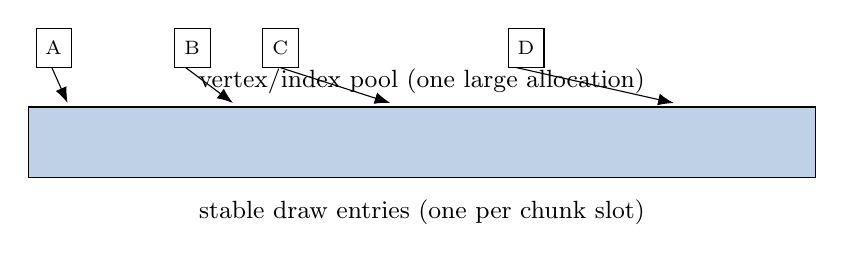
\begin{tikzpicture}[font=\small]
  \fill[accent!10] (0,0) rectangle (10,0.9);
  \foreach \x/\w/\lab in {0/2.2/chunk A,2.2/1.4/chunk B,3.6/2.8/chunk C,6.4/1.1/free,7.5/2.5/chunk D}
    \fill[accent!28] (\x,0) rectangle (\x+\w,0.9)
      node[midway,font=\scriptsize]{\lab};
  \draw (0,0) rectangle (10,0.9);
  \node[above] at (5,0.95) {vertex/index pool (one large allocation)};
  % draw entries
  \foreach \x/\lab in {0/A,2.2/B,3.6/C,7.5/D} {
    \draw (0.1+\x*0.8,1.4) rectangle (0.1+\x*0.8+0.45,1.9);
    \node[font=\scriptsize] at (0.1+\x*0.8+0.22,1.65) {\lab};
  }
  \draw[-{Latex[length=2mm]}] (0.3,1.4)--(0.5,0.95);
  \draw[-{Latex[length=2mm]}] (2.0,1.4)--(2.6,0.95);
  \draw[-{Latex[length=2mm]}] (3.2,1.4)--(4.6,0.95);
  \draw[-{Latex[length=2mm]}] (6.2,1.4)--(8.2,0.95);
  \node[below] at (5,-0.15) {stable draw entries (one per chunk slot)};
\end{tikzpicture}
\caption{Packed pools and stable draw entries.  Chunk spans are packed
best-fit into one large vertex pool and one large index pool; the draw
entry is a stable index into the indirect-command array.  Rebuilding a
chunk replaces only its span.}
\label{fig:pool}
\end{figure}

\subsection{The draw command}

A draw command is
\begin{equation}
\begin{aligned}
  \text{DrawIndexedIndirectCount}(&\text{indexCount},\text{instanceCount}=1,\\
  &\text{firstIndex},\text{vertexOffset}=\text{baseVertex},\\
  &\text{firstInstance}=\text{slot}).
\end{aligned}
\end{equation}
The vertex shader uses \code{gl_InstanceIndex} only for the per-chunk
vegetation/impostor path; the solid terrain vertex is a direct vertex
attribute.  The index stream is chunk-local: every index is a slot number
in the chunk's vertex span, and \code{vertexOffset} rebases it at draw time.

\subsection{Depth and offscreen composition}

Vegetation is rendered to its own color and depth targets on a parallel
async command buffer; the solid pass has a separate depth target.  The
composite pass tests the vegetation depth against the solid scene depth.
This decoupling is why the vegetation pass can use a different render
scale and why it can be skipped on steady-empty frames.  The solid chunks
themselves are drawn in the main solid pass, with a depth prepass and a
shadow cascade.

\subsection{Shadows}

The shadow renderer reuses the same slots and the same hierarchy.  A
cascade cull emits one compacted command per chunk per cascade, reusing the
already-selected LoD stamp from the main cull.  The shadow vertex shader
reads the same 64-byte vertex and index pool.  No second mesh exists.
The cascade copy lists and descriptor-buffer mirror include the brush map
and wind field so the shadow tessellation stage can displace and classify
the surface without a separate descriptor.

\subsection{Ray tracing}

The hybrid ray tracer builds a BLAS over the merged vertex/index pools.  A
chunk's geometry span is referenced directly:
\begin{itemize}
\item vertex buffer = the pool, vertex stride 64;
\item index buffer = the pool, first index = span's first index;
\item geometry flags = opaque or alpha-tested, depending on the material.
\end{itemize}
Because the span is published only after the finalize fence, the BLAS build
never sees partially written vertices.  A chunk rebuild requests a BLAS
refresh; the proxy boxes are used for the water reflection path and for
the fallback when the BLAS is not ready.

\subsection{Material and mapping}

The vertex carries brush, HSV, texture type, and mapping data.  The solid
fragment shader selects the material texture from the brush and the
triplanar/projection mapping from the texture type.  Because the CPU never
computed a vertex, the mapping data must come from the node: the shape
leaf paints it, internal nodes inherit the dominant child, and finalize
writes it into the vertex.  A mapping bug therefore shows up as a texture
scale collapse, not as a geometry error.

\subsection{The frame graph}

The main frame is roughly:
\begin{enumerate}
\item frame fences and pending command-buffer processing;
\item uploads and deferred destroys;
\item GPU cull for solid, water, SDF, bbox, vegetation;
\item depth prepass;
\item shadow cascades;
\item solid color pass;
\item water, vegetation, video, SDF passes;
\item post-process composition;
\item ImGui and present.
\end{enumerate}
The topology pass is not in this list: it runs on worker threads when a
chunk is built, not per frame.  A frame only consumes published spans.

\section{GPU culling and the hole-free LoD gate}
\label{sec:cull}

\subsection{One dispatch, many streams}

The solid \code{IndirectRenderer} owns a single compute dispatch
(\code{IndirectRenderer.comp}) that culls:
\begin{itemize}
\item solid terrain chunks;
\item SDF debug cubes;
\item mesh bounding boxes;
\item main-view vegetation (blade tufts and impostors);
\item three shadow cascades for solid and vegetation.
\end{itemize}
The different streams are appended in the same dispatch and written to
separate outputs.  This avoids one dispatch per stream and keeps the
per-frame CPU cost constant.

\subsection{Frustum test}

The view-projection matrix is a push constant.  The shader extracts six
normalized planes once per workgroup and tests an AABB by its most positive
vertex.  The test is conservative: it can keep a box that is just outside,
but it never rejects a box that intersects the frustum.

\subsection{The hierarchical rung gate}

The LoD gate is the most delicate part of the renderer.  Each published
chunk is a cell of a dyadic ladder.  The goal is to draw exactly one rung
per region, with no holes and no overlaps.  A naive distance-to-centre band
fails because the centres of parent and child are not nested at the same
position; it can reject every rung of a column.

The engine uses the per-entry form of the classic CDLOD recursion.  For an
entry at level $r$ with cell size $L$:
\begin{align}
  L_{\text{base}} &= L/2^r,\\
  R_{\text{self}} &= L_{\text{base}}\cdot\text{bias}\cdot r,\\
  \text{recurseSelf} &= (r>0)\land
    \operatorname{dist}_{\text{AABB}}(\mathbf{c},L) < R_{\text{self}}.
\end{align}
The parent cell is the aligned double-size cube containing the entry.
The parent range is $L_{\text{base}}\cdot\text{bias}\cdot(r+1)$.  The entry
is selected when
\begin{equation}
  \text{recurseParent} \land \lnot\text{recurseSelf},
\end{equation}
with the coarsest rung selected when it does not recurse, and the finest
rung selected whenever its parent recursed (there is nothing finer to
clamp to).  Both distance and range are monotone along the chain, so
exactly one level satisfies the transition for every camera position.

\begin{figure}[htbp]
\centering
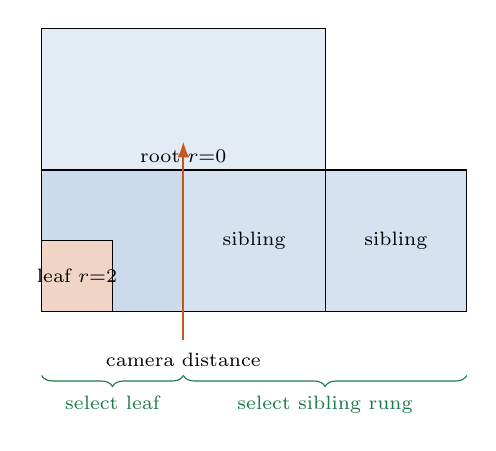
\begin{tikzpicture}[scale=0.9]
  \foreach \x/\y/\s/\lab/\col in {
    0/0/4/root/accent!12,
    0/0/2/child/accent!22,
    0/0/1/leaf/accent2!25,
    2/0/2/sibling/accent!18,
    4/0/2/sibling/accent!18} {
    \fill[\col] (\x,\y) rectangle ++(\s,\s);
    \draw (\x,\y) rectangle ++(\s,\s);
  }
  \node[font=\scriptsize] at (2,2.2) {root $r{=}0$};
  \node[font=\scriptsize] at (0.5,0.5) {leaf $r{=}2$};
  \node[font=\scriptsize] at (3,1) {sibling};
  \node[font=\scriptsize] at (5,1) {sibling};
  \draw[accent2,thick,-{Latex[length=2mm]}] (2,-0.4) -- (2,2.4);
  \node[below,font=\scriptsize] at (2,-0.45) {camera distance};
  \draw[decorate,decoration={brace,mirror,amplitude=4pt},good]
    (0,-0.9)--(2,-0.9) node[midway,below=4pt,font=\scriptsize]{select leaf};
  \draw[decorate,decoration={brace,mirror,amplitude=4pt},good]
    (2,-0.9)--(6,-0.9) node[midway,below=4pt,font=\scriptsize]{select sibling rung};
\end{tikzpicture}
\caption{The hierarchical gate selects one rung per region.  The leaf is
selected near the camera; the sibling rung is selected farther away.  A
region can never lose all rungs because the parent/child ranges are
monotone along the chain.}
\label{fig:gate}
\end{figure}

\subsection{The visible-LoD stamp}

The gate's decision is written into \code{visibleLods[s]} as
\begin{equation}
  \text{stamp} =
  \begin{cases}
    r, & \text{kept},\\
    \texttt{0xFFFFFFFE}, & \text{rejected LoD entry},\\
    \texttt{0xFFFFFFFF}, & \text{no LoD data (legacy)}.
  \end{cases}
\end{equation}
The shadow cascade cull reads this stamp instead of re-deriving the
selection with a stale camera position.  This fixes the old bug where far
chunks cast finest-mesh shadows for a mesh the main pass never drew.

\subsection{Vegetation follows the chunk}

Vegetation is not a separate culling stream.  The per-solid-entry
vegetation table holds the instance count and first instance for the
chunk.  When the solid entry survives the frustum and rung gate, the same
dispatch emits a blade-tuft command and an impostor command for the chunk.
The vegetation bounding box is the chunk AABB, so it is culled exactly with
the terrain.  A chunk with no vegetation has \code{instanceCount=0} and is
skipped.

\subsection{Water pin}

The water stream uses the same gate but pins the finest rung
($r=0$) at every distance.  Small floating water volumes (mirror spheres)
are sub-cell features past rung 2--3; the coarse rungs mesh to nothing and
would leave a hole.  There are few water draws, so finest-always is
affordable.  The shadow, backface, and RT passes follow the same stamp.

\subsection{Indirect count}

The cull writes a compacted command array and a count.  The draw uses the
indirect-count command with the count buffer.  The count is
read back asynchronously for the stats overlay; the draw itself never
waits on the CPU.  The count buffer is reset by \code{vkCmdFillBuffer}
before the dispatch.

\section{GPU-resident effects: grass and fire}
\label{sec:effects}

\subsection{The shared span}

Vegetation and fire both need information from the chunk's surface, but
neither needs a CPU copy of the triangle mesh.  They consume the same
published span:
\begin{itemize}
\item vegetation reads the vertex and index pools directly;
\item fire reads the node SDFs on the host build and emits anchors.
\end{itemize}
Both are keyed by chunk id and both participate in the chunk's lifecycle:
a republish replaces the old data, a delete tombstones it, and a rebuild
creates a new version.

\subsection{Vegetation placement}

The placement shader \code{VegetationPlacement.comp} reads the chunk's
vertex span, treats every triangle as a potential grass emitter, and:
\begin{enumerate}
\item rejects triangles with no grass-brush vertex;
\item computes the triangle area;
\item expands a stochastic number of virtual slots proportional to area;
\item samples a barycentric point;
\item applies the dominant-vertex brush test;
\item applies the biome noise gate;
\item selects a blade variant and a rotation fraction by position hash;
\item writes a 32-byte instance record.
\end{enumerate}
The placement output goes into a scratch ring.  The host reads the accepted
count, allocates an exact persistent buffer, copies the scratch slice, and
publishes the chunk.  No instance byte reaches the host.  A coarse rung
with thousands of tufts is capped at \code{kPlacementScratchPerChunk} to
bound the far-field draw; the cap is a deliberate density reduction, not a
silent overflow.

\subsection{Why not one instance per triangle?}

The old CPU code expanded slots on the CPU, one per area-weighted sample.
The GPU port does the same expansion in the shader: each invocation is one
triangle and loops over its stochastic slot count.  This avoids a
prefix-sum pass and a second dispatch.  The trade-off is that the output
order is non-deterministic; the instance record itself is deterministic
because every random draw is seeded by the chunk, triangle, and slot.

\subsection{The vegetation draw}

The cull emits a blade-tuft command with
\code{indexCount=36} (12 blades, one triangle each) and an impostor command
with \code{indexCount=6}.  The instance count and first instance come from
the per-chunk table.  The vegetation vertex shader reads the instance
record:
\begin{itemize}
\item position,
\item normal,
\item variant and rotation,
\item baked height,
\end{itemize}
and expands the procedural blade geometry.  The impostor path samples the
captured blade atlas and reconstructs depth from the captured depth array.

\subsection{Lava/fire anchors}

The SDF fire effect is driven by brush-4 surfaces.  The old collector
sampled the CPU mesh; after the GPU-only change it received an empty
geometry.  The replacement resolves anchors during the chunk build:
\begin{enumerate}
\item for every brush-4 surface node that owns a vertex slot, evaluate the
  node's trilinear SDF and gradient at its centre;
\item take one Newton step to the zero crossing;
\item clamp to the node cube;
\item emit a position, normal, and seed.
\end{enumerate}
The anchors are carried on \code{LoDMesh} to the main thread and ingested
by \code{SdfRenderer}.  The renderer caps the number per chunk, deduplicates
nested LoD rungs on an 8 m grid, builds a flame instance list, and stages
the SDF scene.  The volumetric fire path then renders the flames through
the same generic SDF scene as smoke and bullets.

\begin{figure}[htbp]
\centering
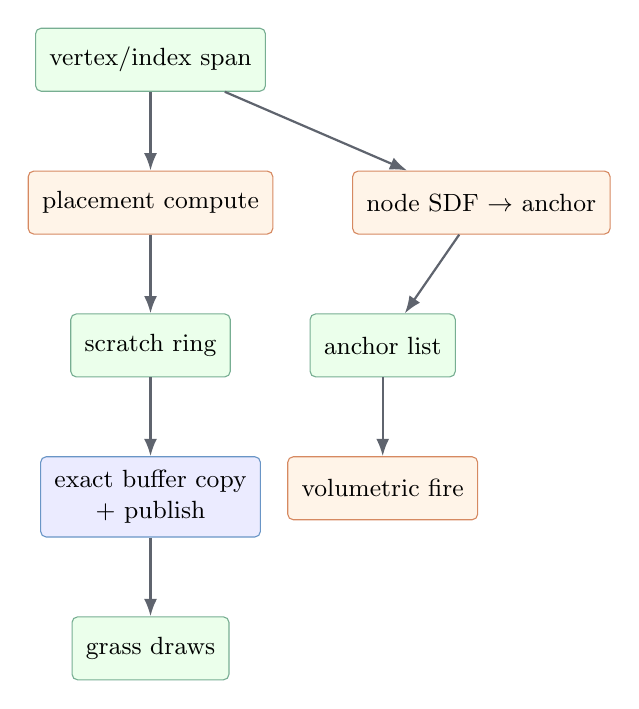
\begin{tikzpicture}[font=\small]
  \node[io] (V) {vertex/index span};
  \node[gpu,below=of V] (veg) {placement compute};
  \node[gpu,right=of veg] (sdf) {node SDF $\to$ anchor};
  \node[io,below=of veg] (scratch) {scratch ring};
  \node[io,right=of scratch] (anchors) {anchor list};
  \node[cpu,below=of scratch] (copy) {exact buffer copy\\+ publish};
  \node[io,below=of copy] (draw) {grass draws};
  \node[gpu,below=of anchors] (fire) {volumetric fire};
  \draw[arrow] (V)--(veg); \draw[arrow] (veg)--(scratch);
  \draw[arrow] (scratch)--(copy); \draw[arrow] (copy)--(draw);
  \draw[arrow] (V)--(sdf); \draw[arrow] (sdf)--(anchors);
  \draw[arrow] (anchors)--(fire);
\end{tikzpicture}
\caption{Two GPU-resident effects sharing the chunk span.  Vegetation
writes instances and copies them to an exact persistent buffer; fire
resolves anchors during the build and hands them to the SDF renderer.}
\label{fig:effects}
\end{figure}

\subsection{Ownership and cleanup}

Both effects register with the chunk lifecycle:
\begin{itemize}
\item a republish replaces the chunk's instance buffer/anchor entry;
\item an empty chunk tombstones the old entry;
\item a chunk delete removes the entry and defers the buffer destroy until
  all pending submissions complete;
\item app shutdown stops the worker pools before the device idle wait.
\end{itemize}
The effect data is therefore never left pointing at a freed span.

\section{Performance and memory}
\label{sec:perf}

\subsection{Cost model}

The per-chunk cost is
\begin{equation}
  C_{\text{chunk}} =
  C_{\text{flatten}} + C_{\text{upload}} + C_{\text{walk}} +
  C_{\text{read}} + C_{\text{reserve}} + C_{\text{finalize}} +
  C_{\text{publish}}.
\end{equation}
The flatten and upload scales with the number of nodes in the
neighbourhood; the walk scales with the number of scan cells and active
edges; the finalize scales with the index and vertex counts.  The host
reads only six integers between the two submissions.

\subsection{Measured topology rates}

The debug profiler in \code{OctreeTopologyCompute} reports cumulative
averages every 256 chunks when \code{VULKAN_SETUP_DIAG=1}.  On the reference
scene the observed windows were:

\begin{center}
\begin{tabular}{@{}rrrr@{}}
\toprule
Chunks & avg ms/chunk & avg cells & avg nodes\\
\midrule
256  & 8.3  & 1031 & 3761\\
512  & 9.3  & 911  & 3440\\
768  & 10.0 & 885  & 3382\\
1280 & 18.9 & 788  & 3053\\
\bottomrule
\end{tabular}
\end{center}

The later window is slower despite fewer cells and nodes because the
workers contend with the render thread and with descriptor/buffer growth.
The uncontended floor reported for the last window of an earlier capture
was about 4.2 ms/chunk.  The difference is a convoy effect, not a
super-linear algorithm.

\begin{figure}[htbp]
\centering
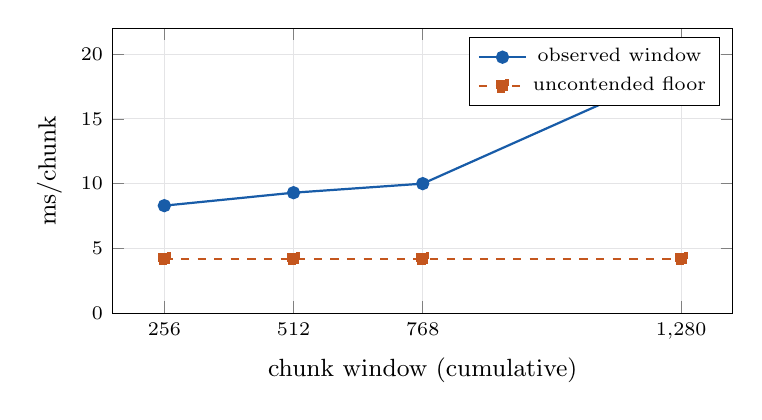
\begin{tikzpicture}
\begin{axis}[
  width=0.78\linewidth,height=5.2cm,
  xlabel={chunk window (cumulative)},ylabel={ms/chunk},
  xtick={256,512,768,1280},
  ymin=0,ymax=22,
  grid=major,grid style={draw=ink!12},
  legend style={font=\scriptsize,at={(0.98,0.97)},anchor=north east},
  tick label style={font=\scriptsize},
  label style={font=\small}
]
\addplot[mark=*,thick,accent] coordinates {(256,8.3) (512,9.3) (768,10.0) (1280,18.9)};
\addplot[mark=square*,thick,accent2,dashed] coordinates {(256,4.2) (512,4.2) (768,4.2) (1280,4.2)};
\legend{observed window, uncontended floor}
\end{axis}
\end{tikzpicture}
\caption{Observed topology cost per chunk.  The floor is the cost when the
worker pool is not contending with the render thread or with buffer
growth.}
\label{fig:perf}
\end{figure}

\subsection{Throughput}

The walk is one invocation per scan cell.  For a chunk with about 900 scan
cells and 3.4k nodes, the measured 8--19 ms includes the host-side flatten
and upload, the two submissions, and the fence wait.  The GPU dispatch
itself is a small fraction: the adaptive walk is branch-heavy and the
per-invocation arrays (break list, stack, memo) are larger than the scan
loop.  The cost is dominated by the branch divergence of the edge
classification and by the break collection, not by the QEF solve.

\subsection{Memory budget}

The reference configuration reserves:
\begin{center}
\begin{tabular}{@{}lrr@{}}
\toprule
Resource & Size & Notes\\
\midrule
Solid vertex pool & 768 MB & 64 B $\times$ 12M elements\\
Solid index pool & 192 MB & 4 B $\times$ 48M elements\\
Water vertex pool & 96 MB & 64 B $\times$ 1.5M elements\\
Water index pool & 96 MB & 4 B $\times$ 24M elements\\
Vegetation concat A/B & 256 MB $\times$ 2 & 8M instances $\times$ 32 B\\
Vegetation baked A/B & 32 MB $\times$ 2 & one float per instance\\
Vegetation scratch & 80 MB & 2 $\times$ 10 $\times$ 131k $\times$ 32 B\\
Texture arrays & 720 / 747 MB & five maps, 28 layers\\
\bottomrule
\end{tabular}
\end{center}

The pools are preallocated once.  A publish only carves or frees a span;
it never allocates a Vulkan buffer.  This is why the steady-state path has
zero \code{vmaCreateBuffer} calls and why a streaming burst cannot
fragment the allocator.

\subsection{Streaming behaviour}

Chunks are drained at a controlled rate (16 per frame in the scene
publisher, 10 per frame for vegetation).  A full drain would submit
hundreds of topology builds at once; on a 4 GB iGPU that trips the amdgpu
watchdog.  The rate limit keeps the submit queue bounded and spreads the
GPU work over frames.  The vegetation and fire effects lag the solid
publish by one or two frames; that is acceptable because the chunk is not
visible until its draw entry is published.

\subsection{Failure costs}

The expensive failure is a key-capacity retry: it re-uploads the node
table and re-runs the walk.  The hint (25 keys per scan cell plus 64) was
calibrated to make retries rare.  The hard cap (8M keys, 32 MB) is chosen
so a pathological chunk fails explicitly rather than allocating
unbounded memory.  A pool exhaustion is a sizing bug: the pools are
preallocated for the worst measured scene, and a new scene must bump the
budget deliberately.

\subsection{Interpretation}

The pipeline is not ``free''.  It pays:
\begin{itemize}
\item a per-chunk flatten and upload of the node neighbourhood;
\item two submissions and one fence wait;
\item a small host read of six counters;
\item a per-chunk span reservation and descriptor update.
\end{itemize}
It saves:
\begin{itemize}
\item a GPU$\rightarrow$CPU vertex readback;
\item a CPU-side QEF solve for every vertex;
\item a host-side triangle append and a staging upload;
\item a CPU-to-GPU copy of the index stream.
\end{itemize}
On a discrete GPU the readback and staging are the dominant costs; on an
integrated GPU they are even more expensive because the memory is shared.
The measured topology cost is the price of the split, and it is paid on
worker threads, not on the render thread.

\section{Correctness invariants and validation}
\label{sec:validation}

\subsection{The invariants}

The following invariants must hold after any change to the pipeline.

\begin{invariant}[Single Cartesian producer]
For a runtime chunk, every Cartesian vertex is written by
\code{OctreeTriangles.comp} stage 1.  No CPU code writes a chunk vertex.
The offline exporter is the only exception and is explicitly marked.
\end{invariant}

\begin{invariant}[Slot determinism]
The host assigns vertex slots in node-table order.  A rebuild with the same
octree revision produces the same slot for the same surface node.
\end{invariant}

\begin{invariant}[Span lifetime]
A draw entry references a span only after the finalize fence has signaled
and the drop counters are zero.  The old span is not freed until the cull
frame that could still reference it has retired.
\end{invariant}

\begin{invariant}[Index locality]
Every index written by stage 1 is a chunk-local slot
$s\in[0,\text{vertexCapacity})$ and is rebased by
\code{vertexOffset=baseVertex} at draw time.
\end{invariant}

\begin{invariant}[Owner consistency]
For a shared edge, both neighbouring chunks select the same owner, sample
the same four quadrants, and emit the same sub-segment list.  The owner
key is global (size, min, node index).
\end{invariant}

\begin{invariant}[Winding oracle]
Triangle winding is derived from the producing cell's corner signs, not
from a QEF normal.  A degenerate owner interpolation falls back to the
producing cell's signs.
\end{invariant}

\begin{invariant}[No silent truncation]
A break-list, stack, key-capacity, or span overflow sets a counter and
fails the chunk.  It never publishes a partial span.
\end{invariant}

\subsection{Validation layers}

Development builds enable Khronos validation, synchronization validation,
best-practices validation, and, when requested, GPU-assisted validation.
The engine treats every validation message as a bug.  The most relevant
checks for this pipeline are:
\begin{itemize}
\item descriptor range and offset alignment;
\item storage-buffer access outside the bound range;
\item synchronization hazards between compute writes and vertex/index
  reads;
\item queue submission threading;
\item image layout transitions in the offscreen vegetation/SDF targets.
\end{itemize}

\subsection{GPU-assisted validation}

GPU-assisted validation instruments shader resource access.  It is
especially useful here because a wrong \code{relVertexBase} or a stale span
may not crash: it reads another chunk's vertex and renders a stretched
triangle.  The GPU-assisted run catches the out-of-range descriptor access
at draw time.  The pass is slow and is used as a targeted check, not as the
default.

\subsection{Self-check against the CPU walker}

A diagnostic mode can rebuild a chunk with the CPU walker and compare the
triangle sets.  The comparison is quantization-tolerant because the GPU
and CPU may differ in the last bits of a QEF solve.  The check is:
\begin{itemize}
\item same triangle count;
\item same set of quantized triangle centroids;
\item same material assignment;
\item vertex deviation below a tolerance.
\end{itemize}
A large deviation indicates a flattening error (wrong cell, wrong LoD,
wrong owner), not a floating-point difference.

\subsection{Determinism tests}

A chunk is built twice from the same revision.  The vertex spans must be
byte-identical and the index stream must be a permutation of the first.
The triangle set is compared order-insensitively.  This catches:
\begin{itemize}
\item an unstable table order;
\item a slot assignment that depends on a hash map iteration;
\item an atomic append that changes the triangle set (it should not).
\end{itemize}

\subsection{Synchronization validation}

The topology pass is checked for:
\begin{itemize}
\item compute$\rightarrow$host visibility before the counter read;
\item compute$\rightarrow$vertex/index visibility before the draw;
\item no read of the pool while a finalize dispatch is still writing;
\item no free of a span still referenced by an in-flight cull.
\end{itemize}
The vegetation copy is checked for the same pattern: placement fence
$\rightarrow$ host read $\rightarrow$ copy submission $\rightarrow$
publish $\rightarrow$ consolidation copy.

\subsection{The queue-threading bug}

A release run produced
\begin{quote}\ttfamily\small\raggedright
vkQueueSubmit2(): THREADING ERROR : object of type VkQueue is\\
simultaneously used...
\end{quote}
The cause was \code{vkDeviceWaitIdle()} running without the submission
mutex while a worker submitted a topology or upload command.  The fix:
\begin{itemize}
\item \code{deviceWaitIdle()} takes the global submit mutex;
\item cleanup stops the CPU pools before the first idle wait.
\end{itemize}
After the fix, a full scene load and shutdown produced no threading or
validation messages.  This is an example of why the synchronization
section is part of the algorithm, not an afterthought.

\subsection{Regression checklist}

Any change to the mesher should run:
\begin{enumerate}
\item a debug build;
\item a load of the reference scene with all effects;
\item a validation scan of \code{logs/run.log};
\item a GPU-assisted run on a small scene;
\item a CPU-vs-GPU self-check on a chunk with a LoD boundary;
\item a rebuild/delete/rebuild cycle on the same chunk id.
\end{enumerate}
If any of these fails, the change is not ready.

\section{Discussion, limitations, and future work}
\label{sec:discussion}

\subsection{What the split buys}

The CPU octree is a semantic store: it knows the SDF, the brush, the
mapping, the version, and the LoD ladder.  The GPU mesher is a pure
function from a flattened neighbourhood to a dual mesh.  This separation
makes both sides simpler:
\begin{itemize}
\item the CPU never needs a triangle mesh to answer ``what is the
  material at this cell?'';
\item the GPU never needs a pointer, an allocator, or a tree lock;
\item the renderer never needs a conversion pass;
\item the exporter can reuse the CPU walker as a reference.
\end{itemize}

\subsection{The remaining host cost}

The host still pays for the flattened upload and the two fence waits per
chunk.  The measured 8--19 ms/chunk is not negligible.  The cost is on
worker threads, so it does not directly stall the render thread, but it
consumes CPU cores and memory bandwidth.  The next step would be to batch
several chunks into one submission and share one descriptor set, as the
perf reports propose.  That would amortize the submit/fence cost and the
descriptor writes.  The current per-chunk design was chosen for
incremental streaming and easy failure isolation; batching is a
throughput optimization, not a correctness requirement.

\subsection{The mesh is not the only consumer}

The same span feeds:
\begin{itemize}
\item the raster solid pass;
\item the shadow cascades;
\item the ray-tracing BLAS;
\item the vegetation placement compute;
\item the SDF fire anchors (via node SDFs).
\end{itemize}
This is why the span protocol is centralized in \code{IndirectRenderer}.
If each consumer allocated its own copy, the memory and the synchronization
surface would explode.  The packed pool is the single source of geometry
truth for the frame.

\subsection{Adaptive LoD and cracks}

The adaptive stitching is exact for the chunk-local walk, but it relies on
both chunks seeing the same four quadrant cells.  The one-cell margin
guarantees this for a neighbour that is at most one cell larger.  A
pathological tree with a much larger neighbour (more than one cell) could
still sample outside the margin.  The flattening uses the largest target
cell in the subtree, not the chunk's own cell, precisely to cover this
case.  A future change that shrinks the margin must re-run the
CPU-vs-GPU self-check on a chunk with a coarse neighbour.

\subsection{The coarse-rung density cap}

Vegetation placement caps a single coarse rung at a fixed instance count.
This is a deliberate visual/performance trade: a root-scale chunk can
request hundreds of thousands of tufts, which is both expensive and
visually indistinguishable from a smaller count at its distance.  The cap
is logged, not silent.  A future distance-density model could replace the
hard cap with a screen-space or distance-based thinning curve.

\subsection{The fire anchors}

The fire effect now derives anchors from the node SDFs rather than from the
triangulated surface.  This is cheaper and fits the GPU-only mesh, but it
is coarser than the old triangle sampling.  The Newton step lands on the
trilinear zero crossing; for a primitive sphere or cylinder this is
accurate.  For a highly non-planar cell, the anchor can be a few
centimetres off the true QEF surface.  The flame scale is large enough
that this is not visible.  A future improvement could run a small GPU
placement pass over the brush-4 triangles and read back only the anchor
records.

\subsection{What would break the design}

The following changes would violate the contract and require a redesign:
\begin{itemize}
\item reading a vertex back to the host (destroys the no-readback
  property);
\item letting the CPU write a chunk vertex (destroys the single-producer
  invariant);
\item freeing a span without a cull-frame delay (use-after-free);
\item changing the node table order without re-running the exporter
  comparison (changes slot assignment and the BLAS);
\item dropping a triangle on overflow instead of failing (silent holes).
\end{itemize}

\subsection{Future work}

Three directions are natural:
\begin{enumerate}
\item \textbf{Batched topology.}  Flatten all chunks of a layer into one
  arena, record one geometry dispatch for the batch, and read all counters
  with one map.  This is the highest-leverage performance change.
\item \textbf{GPU-side fire placement.}  A compute pass over brush-4
  triangles could produce anchors in a device buffer and the SDF scene
  could consume them directly, avoiding the host anchor list.
\item \textbf{Compressed vertex payload.}  The 64-byte vertex is generous;
  a packed normal/brush/mapping format could halve the pool and the
  bandwidth, at the cost of a decode in the vertex shader and the BLAS
  build.
\end{enumerate}

\section{Conclusion}
\label{sec:conclusion}

This report followed one geometric path from an author's implicit shape to
a shaded pixel.  The CPU evaluates the SDF, builds an adaptive octree of
corner samples, simplifies it into a LoD ladder, and flattens a chunk's
neighbourhood into compact tables.  The GPU walks the twelve cube edges,
stitches LoD boundaries, solves one dual vertex per surface cell, and
writes the final 64-byte vertices and chunk-local indices directly into
the renderer's persistent pools.  The host sees counters, slots, and
versions—not vertices.

The key ideas are:
\begin{itemize}
\item \textbf{One Cartesian producer.}  The geometry pass is the only runtime code
  that writes a vertex.  This eliminates an entire class of
  CPU/GPU divergence and makes the offline exporter a meaningful
  reference.
\item \textbf{Root-consistent flattening.}  The GPU table is a
  serialisable snapshot of the exact neighbourhood the CPU walker would
  traverse, including the one-cell margin for coarse neighbours.
\item \textbf{Break-based stitching.}  The edge is split at every cell
  boundary, not at a fixed table of configurations.  Two chunks resolve
  the same edge to the same owner and the same sub-segments.
\item \textbf{Span publishing.}  A chunk's geometry is a reserved range in
  a large pool, published only after the geometry fence and freed only
  after the cull frames that could reference it have retired.
\item \textbf{One hierarchy for everything.}  Raster, shadows, ray
  tracing, vegetation, and fire all consume the same published span or the
  same node metadata.
\end{itemize}

The result is not a toy mesher.  It streams an adaptive, crack-free
surface from a mutable SDF octree into a real-time renderer without a
vertex readback, and it keeps the host's work proportional to the number
of chunks and nodes, not to the number of triangles.  The measured costs
and the invariants in this report are the contract a future change must
preserve.

\appendix
\section{Storage layouts and constants}
\label{app:layout}

\subsection{Octree node record (host)}

\begin{center}
\begin{tabular}{@{}lll@{}}
\toprule
Field & Type & Bytes\\
\midrule
\code{sdf[8]} & float & 32\\
\code{brushIndex} & int & 4\\
\code{textureType} & int & 4\\
\code{data} & vec2 & 8\\
\code{hsv} & vec3 & 12\\
\code{blockId} & uint & 4\\
\code{bits} & uint8 & 1\\
\code{lod} & uint8 & 1\\
\code{chunkLod} & uint8 & 1\\
\code{version} & uint & 4\\
\bottomrule
\end{tabular}
\end{center}

\subsection{GPU node table (flattened)}

\begin{center}
\begin{tabular}{@{}lll@{}}
\toprule
Binding & Record & Bytes\\
\midrule
0 & \code{vec4 sdf0} & 16\\
1 & \code{vec4 sdf1} & 16\\
2 & \code{vec4 cubeMinSize} & 16\\
3 & \code{ivec4 meta} & 16\\
4 & \code{vec4 nodeHsv[2]} & 32\\
5 & \code{ivec4 child03} & 16\\
6 & \code{ivec4 child47} & 16\\
\midrule
total & & 128\\
\bottomrule
\end{tabular}
\end{center}

\subsection{Packed vertex record}

\begin{center}
\begin{tabular}{@{}lll@{}}
\toprule
Word & Field & Bytes\\
\midrule
0 & position.xyz + color.x & 16\\
1 & color.yz + texCoord.xy & 16\\
2 & normal.xyz + brush bits & 16\\
3 & textureType bits + hsv & 16\\
\midrule
total & & 64\\
\bottomrule
\end{tabular}
\end{center}

\subsection{Push constants}

\begin{center}
\begin{tabular}{@{}ll@{}}
\toprule
Field & Meaning\\
\midrule
\code{cellCount} & scan cells in this dispatch\\
\code{targetLod} & rung to scan\\
\code{fromId} & descent anchor\\
\code{fromBrush} & fallback brush\\
\code{rootMinSize} & world root $(x,y,z,L)$\\
\code{worldSize} & root edge for epsilon\\
\code{keyCapacity} & raw key bound\\
\code{pass} & 0 walk / 1 finalize\\
\code{vertexBase} & span-relative vertex base\\
\code{vertexCapacity} & vertex span bound\\
\code{indexBase} & span-relative index base\\
\code{indexCapacity} & index span bound\\
\code{indexCount} & raw vertices to remap\\
\code{nodeCount} & node-table entries to write\\
\code{diag} & diagnostic counters on/off\\
\bottomrule
\end{tabular}
\end{center}

\subsection{Constants}

\begin{center}
\begin{tabular}{@{}lll@{}}
\toprule
Name & Value & Purpose\\
\midrule
\code{kVerticesPerCellHint} & 25 & key sizing\\
\code{kKeyCapacityHeadroom} & 64 & key sizing\\
\code{kMaxKeysPerCall} & $2^{23}$ & hard key cap\\
\code{BREAK\_CAP} & 64 & final breaks per edge\\
\code{LOCAL\_BREAK\_CAP} & 32 & local breaks per interval\\
\code{TASK\_STACK} & 256 & interval stack\\
\code{POS\_MEMO} & 8 & QEF memo\\
\code{kInstanceStride} & 32 & vegetation instance\\
\code{kMaxVegChunks} & 4096 & vegetation chunk cap\\
\code{kPlacementScratchPerChunk} & 131072 & vegetation coarse cap\\
\bottomrule
\end{tabular}
\end{center}

\section{The complete scan-cell algorithm}
\label{app:algorithm}

\begin{algorithm}[H]
\caption{GPU scan cell (one invocation per cell)}
\begin{algorithmic}[1]
\State $cell \gets$ cell descriptor from table
\State $corners[8] \gets$ node SDF samples
\For{$e=0$ to $11$}
  \State $(i,j) \gets$ \code{EDGES}[e]
  \If{sign($corners[i]$) $=$ sign($corners[j]$)}
    \State \textbf{continue}
  \EndIf
  \State $span \gets$ \code{makeEdgeSpan}(e, cell)
  \If{$span.end-span.start \le 2\epsilon$}
    \State \textbf{continue}
  \EndIf
  \State $breaks \gets \{span.start, span.end\}$
  \State \code{collectBreaks}(span, span.start, span.end)
  \If{overflow} \State \textbf{fail chunk} \EndIf
  \State sort/unique($breaks$)
  \For{$k=1$ to $|breaks|-1$}
    \If{$breaks[k]-breaks[k-1] > 2\epsilon$}
      \State \code{emitSegment}(span, $breaks[k-1]$, $breaks[k]$,
        $sign_i$, $sign_j$)
    \EndIf
  \EndFor
\EndFor
\end{algorithmic}
\end{algorithm}

\section{Glossary}
\label{app:glossary}

\begin{description}[leftmargin=2.2em,style=nextline]
\item[Chunk] A cube of edge $\Delta$ whose subtree is flattened and meshed
  as one unit.  A chunk root is published as a draw entry.
\item[Rung] A level of the chunk ladder.  $r=0$ is the finest published
  level; larger $r$ are coarser ancestors.
\item[Scan cell] A cube at the target rung whose twelve edges are scanned
  for sign changes.
\item[Edge span] The interval of an active cube edge, with its fixed
  coordinates and epsilon.
\item[Break] A coordinate inside an edge span where a neighbouring cell
  boundary forces a split.
\item[Owner] The surface cell that determines the winding and leads the
  ring of a sub-segment.
\item[Raw key] The node index of one triangle corner, written in stage 0
  and remapped to a slot in stage 1.
\item[Slot] The dense vertex index assigned to a surface node by the host.
\item[Span] A reserved range in the packed vertex/index pools.
\item[Stamp] The per-entry LoD keep/reject decision written by the cull and
  consumed by the shadow/RT paths.
\end{description}

\begin{thebibliography}{99}

\bibitem{lorensen87}
W.~E. Lorensen and H.~E. Cline.
\newblock Marching cubes: A high resolution 3D surface construction algorithm.
\newblock \emph{ACM SIGGRAPH Computer Graphics}, 21(4):163--169, 1987.

\bibitem{ju02}
T.~Ju, F.~Losasso, S.~Schaefer, and J.~Warren.
\newblock Dual contouring of Hermite data.
\newblock \emph{ACM Transactions on Graphics (SIGGRAPH)}, 21(3):339--346, 2002.

\bibitem{gibson98}
S.~F.~F. Gibson.
\newblock Constrained elastic surface nets: Generating smooth surfaces from
  binary segmented data.
\newblock In \emph{Proc. MICCAI}, pages 888--898, 1998.

\bibitem{hart96}
J.~C. Hart.
\newblock Sphere tracing: A geometric method for the antialiased ray tracing of
  implicit surfaces.
\newblock \emph{The Visual Computer}, 12(10):527--545, 1996.

\bibitem{quilez}
I.~Quilez.
\newblock Smooth minimum.
\newblock \url{https://iquilezles.org/articles/smin/}, 2013.

\bibitem{cdlod}
S.~Strugar.
\newblock Continuous distance-dependent level of detail for rendering
  heightmaps.
\newblock \emph{Journal of Graphics, GPU, and Game Tools}, 14(4):57--74, 2009.

\bibitem{vulkan}
Khronos Group.
\newblock \emph{Vulkan 1.4 Specification}.
\newblock \url{https://www.khronos.org/registry/vulkan/}, 2024.

\bibitem{ericson}
C.~Ericson.
\newblock \emph{Real-Time Collision Detection}.
\newblock Morgan Kaufmann, 2004.

\bibitem{glm}
G-Truc Creation.
\newblock \emph{OpenGL Mathematics (GLM)}.
\newblock \url{https://glm.g-truc.net/}, 2024.

\bibitem{sdf}
J.~C. Hart, D.~Sandberg, and S.~M. Omohundro.
\newblock Ray tracing implicit surfaces.
\newblock In \emph{SIGGRAPH Course Notes}, 1993.

\end{thebibliography}


\end{document}
